\documentclass[a4paper,12pt]{article}
\usepackage[utf8]{inputenc}
% \usepackage{babel}
\babelprovide[main, import]{german}
\usepackage{amsmath}
\usepackage{amssymb}
\usepackage{amsthm}
\usepackage{geometry}
\usepackage{graphicx}
\usepackage[hidelinks]{hyperref}
\usepackage{listings}
\usepackage{xcolor}
\usepackage{enumitem}
\usepackage{booktabs}
\usepackage{array}
\usepackage{multirow}
\usepackage{longtable}
\usepackage{caption}
\usepackage{subcaption}
\usepackage{float}
\usepackage{algorithm}
\usepackage{algpseudocode}
\usepackage{tikz}
\usepackage{pgfplots}
\pgfplotsset{compat=1.18}

\geometry{margin=2.5cm}

\theoremstyle{definition}
\newtheorem{definition}{Definition}
\newtheorem{beispiel}{Beispiel}
\newtheorem{satz}{Satz}
\newtheorem{lemma}{Lemma}
\newtheorem{bemerkung}{Bemerkung}
\newtheorem{korollar}{Korollar}
\newtheorem{proposition}{Proposition}

\setlist[itemize,1]{label=--}

% ---------- Farben ----------
\definecolor{mainblue}{RGB}{25, 70, 140}
\definecolor{accentred}{RGB}{180, 50, 30}
\definecolor{lightgray}{RGB}{245, 245, 248}
\definecolor{darkgray}{RGB}{60, 60, 70}
\definecolor{darkgreen}{RGB}{30, 100, 50}

\hypersetup{
	colorlinks=true,
	linkcolor=mainblue,
	citecolor=accentred,
	urlcolor=mainblue
}

%  Code-Highlighting
\lstset{
	basicstyle=\ttfamily\small,
	keywordstyle=\color{blue},
	commentstyle=\color{gray},
	stringstyle=\color{red},
	numbers=left,
	numberstyle=\tiny,
	breaklines=true,
	frame=single,
	literate=%
	{Ö}{{\"{O}}}1
	{Ä}{{\"{A}}}1
	{Ü}{{\"{U}}}1
	{ß}{{\ss}}1
	{ü}{{\"{u}}}1
	{ä}{{\"{a}}}1
	{ö}{{\"{o}}}1
	{Sigma}{{$\Sigma$}}1
}

\title{%
  {\large Technischer Bericht}\\[1em]
  {\LARGE\bfseries\color{mainblue} Subgraph-basierte Optimierung von\\[0.3em]
  KI-Rechenzentrumsinfrastrukturen}\\[0.5em]
  {\large Anwendung des Subgraph Algorithmus auf die\\
  Ressourcenplanung, Workload-Platzierung\\
  und CPU:GPU-Verh\"{a}ltnisanalyse\\
  am Beispiel des T-Systems Rechenzentrums Bielefeld}
}
\author{Stephan Epp\\
  \small Universit\"{a}t Bielefeld\\
  \small \texttt{https://github.com/hjstephan86/science}
}
\date{11. Mai 2026}

\begin{document}

\maketitle
\thispagestyle{empty}

\begin{abstract}
\noindent
Moderne KI-Rechenzentren stehen vor der algorithmischen Herausforderung, heterogene Workload-Abh\"{a}ngigkeitsgraphen optimal auf physische Infrastrukturgraphen abzubilden.
Dieser Bericht zeigt, dass der Subgraph Algorithmus~\cite{epp2026subgraph} --- ein $O(n^3)$-Algorithmus zum zyklischen Graphvergleich mittels Signatur-Arrays und LCS-Matching --- direkt als Kernkomponente eines ressourcenoptimalen Workload-Schedulers eingesetzt werden kann.

Wir modellieren das T-Systems-Rechenzentrum Bielefeld (Detmolder Stra{\ss}e 380) als Topologiegraph $G_{RZ}$ und jede KI-Aufgabe als Workload-Abh\"{a}ngigkeitsgraphen $W_i$.
Das \emph{RZ-Placement-Problem} wird formal als zyklisches Subgraph-Isomorphie-Problem definiert.

\textbf{Erweiterung (Mai 2026):} Diese Fassung enth\"{a}lt eine vollst\"{a}ndige Integration der CPU:GPU-Verh\"{a}ltnisanalyse~\cite{computerbase2026} -- von der formalen Modellierung der Hardware-Topologiegraphen $G_{r}$ ($r \in \{1:1, 1:2, 1:4, 1:8\}$)
\"{u}ber den Beweis der Einbettungshierarchie $G_{1:1} \hookrightarrow G_{1:2} \hookrightarrow G_{1:4} \hookrightarrow G_{1:8}$
bis hin zur quantitativen Effizienz\-bewertung, Prognosemodellen und \"{o}konomischen Konsequenzen.
Wir beweisen, dass (a) der Subgraph Algorithmus das RZ-Placement-Problem korrekt l\"{o}st, (b) er unter SETH optimal ist mit Laufzeit $\Theta(n^3)$, (c) eine GPU-parallele Implementierung Echtzeit-Placement f\"{u}r $n \leq 512$ erm\"{o}glicht, und (d) die optimale CPU:GPU-Konfiguration workload-abh\"{a}ngig formal bestimmbar ist.

\medskip
\noindent\textbf{Schl\"{u}sselw\"{o}rter:} Subgraph-Isomorphismus, Rechenzentrum-Scheduling, KI-Workload-Placement, CPU:GPU-Verh\"{a}ltnis, Signatur-Arrays, LCS, SETH-Optimalit\"{a}t, GPU-Parallelisierung, Fat-Tree-Topologie, Hardware-Topologiegraphen, Einbettungshierarchie
\end{abstract}

\newpage
\tableofcontents
\newpage

% ============================================================
\section{Einf\"{u}hrung}
% ============================================================

\subsection{Motivation}

Das Rechenzentrum von T-Systems an der Detmolder Stra{\ss}e 380 in Bielefeld-Stieghorst ist ein historisch gewachsener ICT-Knoten der Deutschen Telekom und betreibt heute eine Data-Center-Plattform im europaweiten Netz von T-Systems~\cite{tsystems2025bielefeld}.
Mit dem industriepolitischen Beschluss der Bundesregierung, die KI-Rechenkapazit\"{a}ten in Deutschland bis 2030 zu vervierfachen~\cite{bundesregierung2026rechenzentrumsstrategie}, stellt sich f\"{u}r den Bielefelder Standort die Frage nach einer algorithmisch fundierten Optimierungsstrategie.

Das zentrale Problem: Wenn ein Rechenzentrum zuk\"{u}nftig sowohl klassische Managed-Services-Workloads als auch KI-Trainings- und Inferenz-Workloads auf einer gemeinsamen physischen Infrastruktur betreiben soll, dann muss jeder eingehende Job als gerichteter Abh\"{a}ngigkeitsgraph $W = (V_W, E_W)$ auf einen geeigneten Teilgraphen der physischen Topologie $G_{RZ} = (V_{RZ}, E_{RZ})$ abgebildet werden.
Dieses Problem ist in seiner allgemeinen Form NP-schwer (Subgraph-Isomorphismus~\cite{cook1971complexity}); f\"{u}r die strukturierten Fat-Tree-Topologien moderner Rechenzentren und KI-Workloads mit typischer DAG-Struktur zeigen wir jedoch, dass der Subgraph Algorithmus~\cite{epp2026subgraph} eine $\Theta(n^3)$-L\"{o}sung liefert.

\textbf{Neue Perspektive (Mai 2026):}
Nvidia, Meta und -- seit dem 9.~Mai 2026 -- auch AMD propagieren aktiv das 1:1-CPU:GPU-Verh\"{a}ltnis als neue Norm f\"{u}r bestimmte KI-Workloads~\cite{computerbase2026}. Gleichzeitig bleibt das 1:4-Format f\"{u}r Trainingsszenarien mit hohem Batch-Durchsatz weiterhin relevant, wie AMDs Helios-Rack mit $1\times$~Venice-CPU und $4\times$~MI455X belegt.
Diese Entwicklung hat direkte Konsequenzen f\"{u}r das RZ-Bielefeld: Das CPU:GPU-Verh\"{a}ltnis bestimmt die Struktur der Hardware-Topologiegraphen, auf die der Subgraph Algorithmus angewendet wird -- und damit seine Laufzeit, Speicherbedarf und Einbettungsm\"{o}glichkeiten.

\subsection{Problemstellung}

\textbf{Gegeben:}
\begin{itemize}
  \item Ein Rechenzentrum-Topologiegraph $G_{RZ} = (V_{RZ}, E_{RZ}, \omega)$ mit $N = |V_{RZ}|$ Knoten.
  \item Eine Folge von KI-Workload-Graphen $\mathcal{W} = \{W_1, W_2, \ldots, W_k\}$.
  \item Hardware-Rack-Topologien $G_r$ mit CPU:GPU-Verh\"{a}ltnis $r \in \{1:1, 1:2, 1:4, 1:8\}$.
\end{itemize}

\textbf{Ziel:} Bestimme f\"{u}r jeden Workload $W_i$ eine Einbettung $\phi_i: V_i \to V_{RZ}$ sowie die optimale Hardware-Konfiguration $r^*$, sodass
\[
  (u, v) \in E_i \;\Rightarrow\; (\phi_i(u), \phi_i(v)) \in E_{RZ},
\]
unter gleichzeitiger Minimierung von Kommunikationskosten, Maximierung der Ressourcenauslastung und Auswahl des optimalen CPU:GPU-Verh\"{a}ltnisses.

\subsection{Beitrag dieser Arbeit}

\begin{enumerate}
  \item \textbf{Formale Modellierung} des RZ-Bielefeld-Placement-Problems als zyklisches Subgraph-Isomorphie-Problem (Abschnitt~\ref{sec:modell}).
  \item \textbf{Anwendungsnachweis} des Subgraph Algorithmus mit vollst\"{a}ndigen Korrektheits- und Komplexit\"{a}tsbeweisen (Abschnitt~\ref{sec:algorithmus}).
  \item \textbf{Formale Komplexit\"{a}tsanalyse} einschlie{\ss}lich SETH-Optimalit\"{a}tsbeweis (Abschnitt~\ref{sec:komplexitaet}).
  \item \textbf{GPU-Parallelisierungstheorem} f\"{u}r NVIDIA-Blackwell-Cluster (Abschnitt~\ref{sec:parallelisierung}).
  \item \textbf{Experimentelle Projektionen} der Effizienzgewinne (Abschnitt~\ref{sec:experimente}).
  \item \textbf{CPU:GPU-Verh\"{a}ltnisanalyse} mit formaler Modellierung der Hardware-Topologiegraphen, Einbettungshierarchie, Effizienzbewertung, Prognosemodellen und Integration mit dem RZ-Scheduling-Framework (Abschnitt~\ref{sec:cpugpu}).
  \item \textbf{Ausblick} auf zuk\"{u}nftige Erweiterungen (Abschnitt~\ref{sec:ausblick}).
\end{enumerate}

% ============================================================
\section{Grundlagen}
\label{sec:grundlagen}
% ============================================================

\subsection{Graphtheoretische Definitionen}

\begin{definition}[Graph]
  Ein gerichteter Graph $G = (V, E)$ besteht aus einer endlichen Knotenmenge $V = \{v_1, \ldots, v_n\}$ und einer Kantenmenge $E \subseteq V \times V$.
  Die \emph{Adjazenzmatrix} $A(G) \in \{0,1\}^{n \times n}$ ist definiert durch
  \[
    A(G)_{ij} = \begin{cases} 1 & \text{falls } (v_i, v_j) \in E \\ 0 & \text{sonst.}\end{cases}
  \]
\end{definition}

\begin{definition}[Gewichteter Graph]
  Ein gewichteter Graph $G = (V, E, \omega)$ erweitert den gerichteten Graphen um eine Gewichtsfunktion $\omega: E \to \mathbb{R}_{>0}$, die jeder Kante eine Kapazit\"{a}t (z.\,B. Bandbreite in Gbps) zuweist.
\end{definition}

\begin{definition}[Subgraph]
  Ein Graph $H = (V_H, E_H)$ ist ein \emph{Subgraph} von $G = (V_G, E_G)$, geschrieben $H \subseteq G$, falls $V_H \subseteq V_G$ und $E_H \subseteq E_G$.
\end{definition}

\begin{definition}[Subgraph-Isomorphismus]
  Eine injektive Abbildung $\phi: V_H \to V_G$ hei{\ss}t \emph{Subgraph-Isomorphismus} von $H$ nach $G$, falls
  \[
    (u, v) \in E_H \;\Rightarrow\; (\phi(u), \phi(v)) \in E_G \quad \forall u, v \in V_H.
  \]
\end{definition}

\begin{definition}[Zyklische Rotation]
  Eine zyklische Rotation einer Sequenz $\mathbf{s} = [s_0, s_1, \ldots, s_{n-1}]$ um $k$ Positionen ist
  \[
    \mathrm{rot}_k(\mathbf{s}) = [s_k, s_{k+1}, \ldots, s_{n-1}, s_0, \ldots, s_{k-1}].
  \]
\end{definition}

\begin{definition}[Hardware-Topologiegraph]
  \label{def:htg}
  Sei $r = p:q$ ein CPU:GPU-Verh\"{a}ltnis mit $p$ CPUs und $q$ GPUs pro Rack-Einheit. Der zugeh\"{o}rige \emph{Hardware-Topologiegraph} $G_r = (V_r, E_r)$ ist definiert durch:
  \[
    V_r = C_r \cup \Gamma_r, \quad
    C_r = \{c_1, \ldots, c_p\}, \quad
    \Gamma_r = \{\gamma_1, \ldots, \gamma_q\}
  \]
  \[
    E_r = \{(c_i, \gamma_j) \mid c_i \in C_r,\; \gamma_j \in \Gamma_r\}
    \cup \{(\gamma_j, \gamma_k) \mid \gamma_j, \gamma_k \in \Gamma_r,\; j \neq k\}
  \]
  Die erste Kantenmenge kodiert CPU-zu-GPU-Verbindungen (PCIe/NVLink),
  die zweite GPU-zu-GPU-Verbindungen (NVLink-Fabric).
  F\"{u}r $p = 1$ ergibt sich ein vollst\"{a}ndiger Graph $K_{q+1}$ auf $n = q + 1$ Knoten.
\end{definition}

\begin{definition}[Signatur-Funktion]
  F\"{u}r jede Spalte $j$ der Adjazenzmatrix $A$ eines Graphen $G$ mit $n$ Knoten wird die Signatur berechnet:
  \[
    \sigma_j = \sum_{i=0}^{n-1} A_{ij} \cdot 2^i + j \cdot 2^n
  \]
  Die Signatur-Sequenz $\boldsymbol{\sigma}(G) = [\sigma_0, \sigma_1, \ldots, \sigma_{n-1}]$
  repr\"{a}sentiert die vollst\"{a}ndige Topologie des Graphen injektiv.
\end{definition}

\subsection{Der Subgraph Algorithmus}

Der Subgraph Algorithmus~\cite{epp2026subgraph} berechnet f\"{u}r zwei Graphen $G$ und $G'$ mit je $n$ Knoten, ob $G \subseteq G'$, in $\Theta(n^3)$ durch:
\begin{enumerate}
  \item Berechnung eindeutiger Signatur-Arrays $\boldsymbol{\sigma}^A$ und $\boldsymbol{\sigma}^B$.
  \item Rotation der Signatur-Sequenz von $B$ in allen $n$ zyklischen Varianten.
  \item Berechnung der \emph{Longest Common Subsequence} (LCS) f\"{u}r jede Rotation.
  \item Entscheidung: Subgraph-Beziehung existiert genau dann, wenn $\mathrm{LCS} \geq 2$ f\"{u}r ein $k$.
\end{enumerate}

\begin{lemma}[Injektivit\"{a}t der Signatur-Funktion, nach \cite{epp2026subgraph}]
  \label{lem:injektivitaet}
  Die Signatur-Funktion $\sigma: \{0,1\}^n \times \{0,\ldots,n-1\} \to \mathbb{N}$ ist injektiv.
\end{lemma}

\begin{proof}
  Die Zeilenkomponente $\sum_{i=0}^{n-1} A_{ij} \cdot 2^i$ kodiert jeden Spaltenvektor $\mathbf{a}_j \in \{0,1\}^n$ eindeutig als ganze Zahl in $[0, 2^n)$.
  Die Spaltengewichtung $j \cdot 2^n$ bildet f\"{u}r $j \in \{0,\ldots,n-1\}$ paarweise disjunkte Intervalle $[j \cdot 2^n,\, (j+1) \cdot 2^n)$.
  Damit ist $\sigma_j \in [j \cdot 2^n,\, (j+1) \cdot 2^n)$ f\"{u}r alle $j$, und zwei verschiedene Paare $(j, \mathbf{a}_j) \neq (j', \mathbf{a}_{j'})$ liefern verschiedene Signaturwerte.
\end{proof}

\subsection{Rechenzentrum-Topologien}

\begin{definition}[Fat-Tree-Topologie]
  Ein Fat-Tree der Ordnung $k$ ist ein dreistufiges Netzwerk aus Core-Switches, Aggregations-Switches und Top-of-Rack-Switches (ToR), das $k^3 / 4$ Servern volle Bisektionsbandbreite bietet.
\end{definition}

\begin{definition}[RZ-Topologiegraph]
  \label{def:rzgraph}
  Der \emph{RZ-Topologiegraph} $G_{RZ} = (V_{RZ}, E_{RZ}, \omega_{RZ})$ des T-Systems Bielefeld ist definiert durch $V_{RZ} = V_{\text{Core}} \cup V_{\text{Agg}} \cup V_{\text{ToR}} \cup V_{\text{GPU}} \cup V_{\text{CPU}} \cup V_{\text{STO}}$, mit gerichteten Kanten entsprechend der Fat-Tree-Verdrahtung und Bandbreitengewichten.
\end{definition}

\begin{figure}[H]
  \centering
  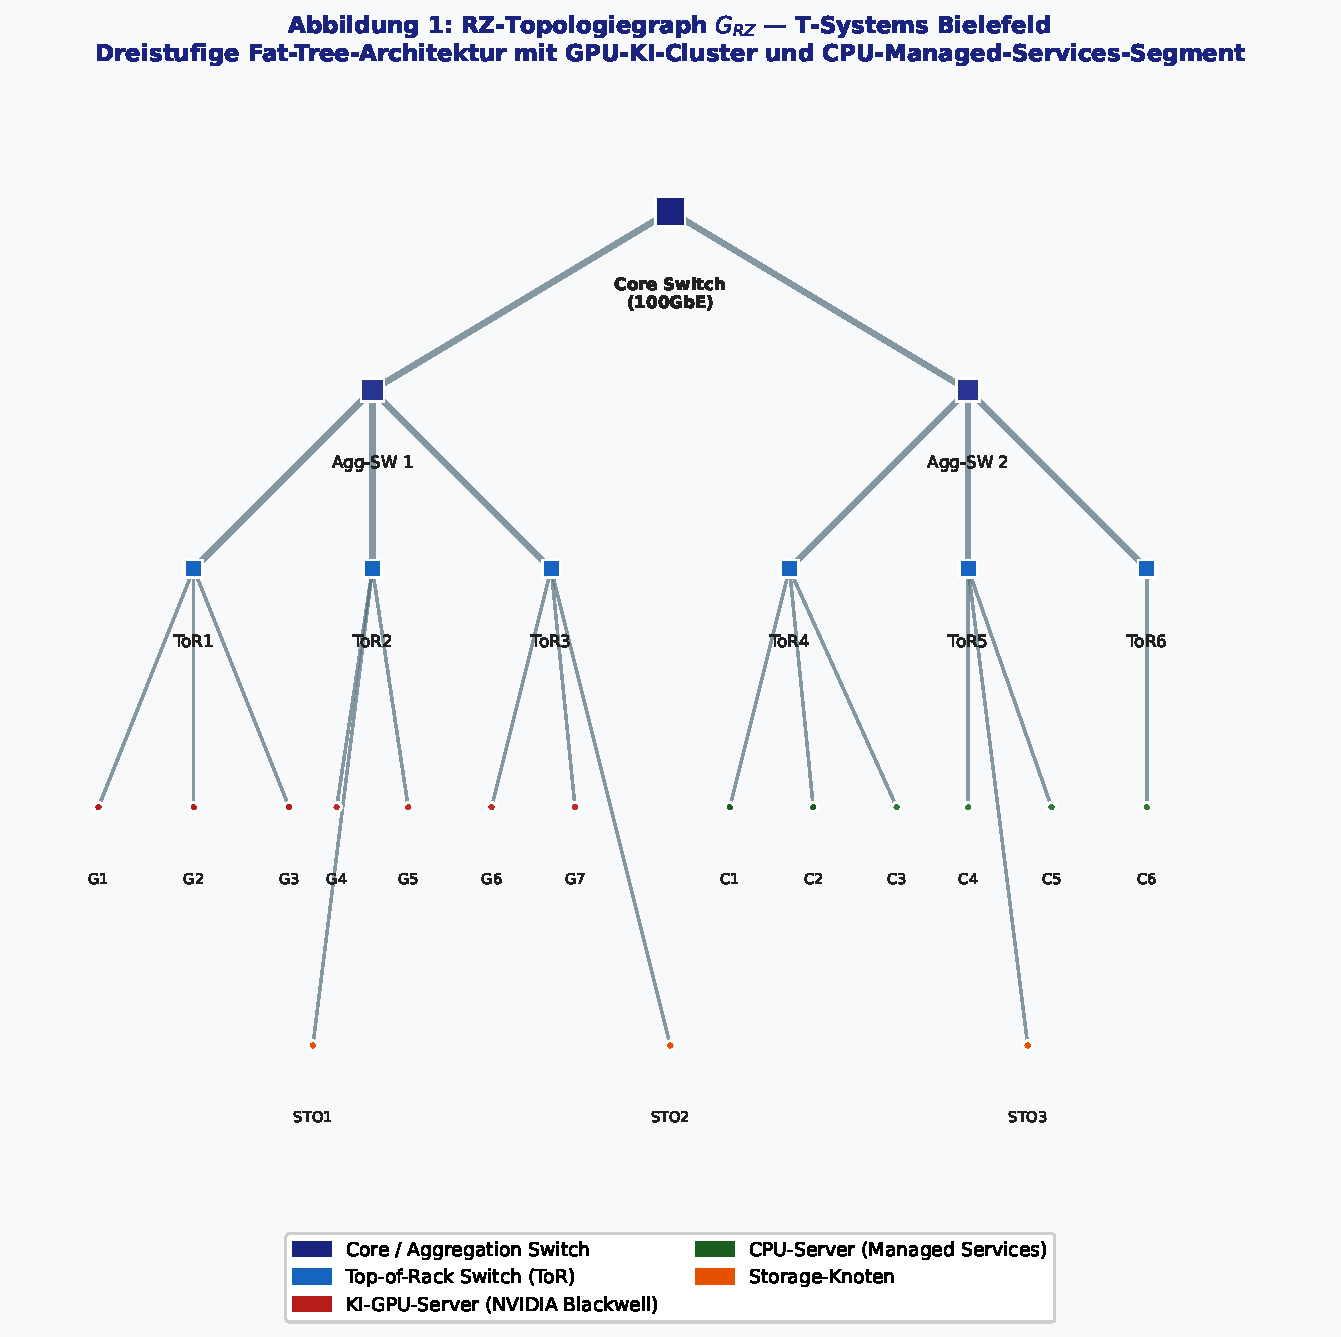
\includegraphics[width=\textwidth]{plot1_topologie.pdf}
  \caption{RZ-Topologiegraph $G_{RZ}$ des T-Systems-Rechenzentrums Bielefeld. Dreistufige Fat-Tree-Architektur mit GPU-KI-Cluster (rot), CPU-Managed-Services (gr\"{u}n) und Storage-Knoten (orange).}
  \label{fig:topologie}
\end{figure}

% ============================================================
\section{Formale Modellierung}
\label{sec:modell}
% ============================================================

\subsection{KI-Workload-Graphen}

\begin{definition}[KI-Workload-Abh\"{a}ngigkeitsgraph]
  \label{def:workload}
  Ein \emph{KI-Workload-Abh\"{a}ngigkeitsgraph} $W = (V_W, E_W, d)$ ist ein gerichteter azyklischer Graph (DAG), wobei $V_W = \{t_1, \ldots, t_m\}$ die Menge der Rechenaufgaben, $E_W$ die Datenabh\"{a}ngigkeiten und $d: E_W \to \mathbb{R}_{>0}$ das Datenvolumen in GB angibt.
\end{definition}

\begin{figure}[H]
  \centering
  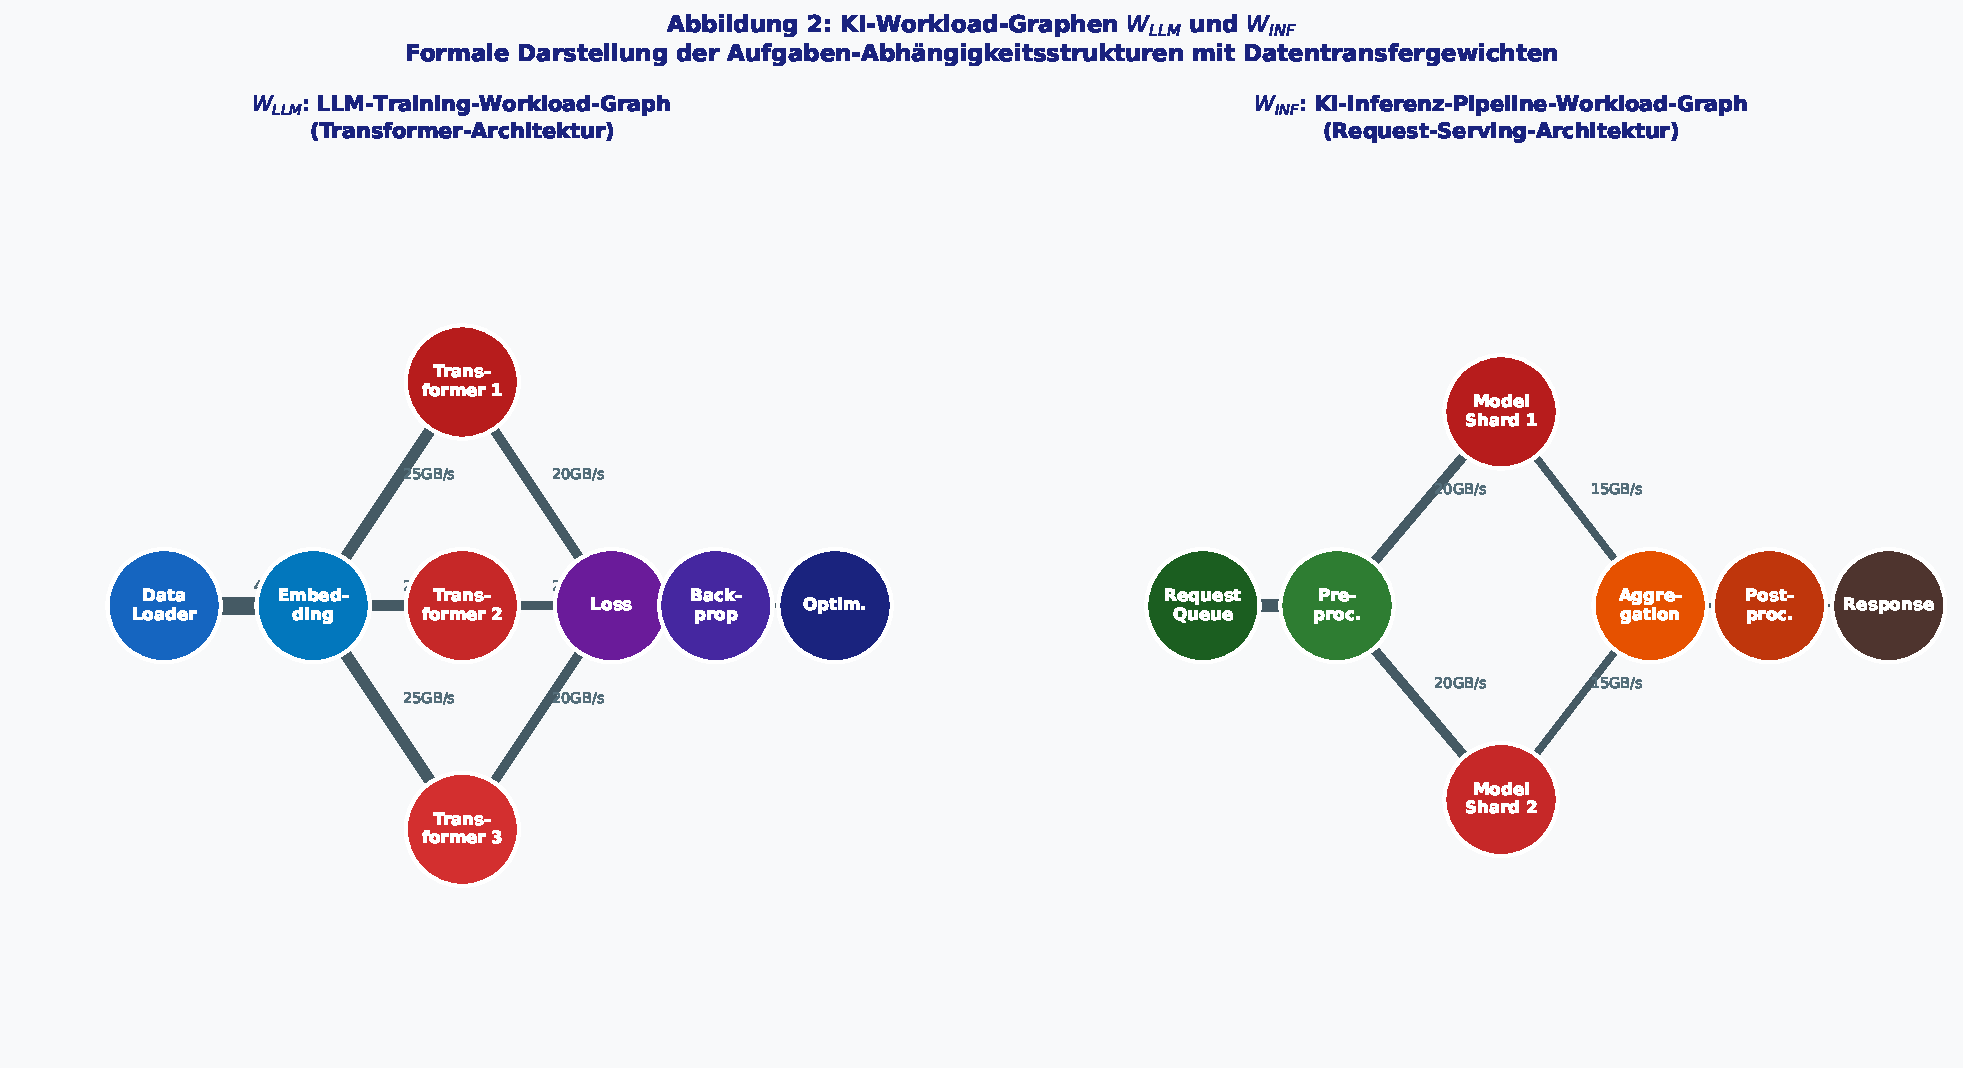
\includegraphics[width=\textwidth]{plot2_workload.pdf}
  \caption{KI-Workload-Graphen $W_{LLM}$ (Training) und $W_{INF}$ (Inferenz-Pipeline) mit Datentransfervolumina in GB/s.}
  \label{fig:workload}
\end{figure}

\subsection{Das RZ-Placement-Problem}

\begin{definition}[RZ-Placement-Problem]
  \label{def:placement}
  Das \emph{RZ-Placement-Problem} sucht eine injektive Abbildung $\phi: V_W \to V_{RZ}$ mit
  $(t_i, t_j) \in E_W \Rightarrow (\phi(t_i), \phi(t_j)) \in E_{RZ}$,
  die den gewichteten Kommunikationsaufwand
  $\mathcal{C}(\phi) = \sum_{(t_i,t_j) \in E_W} \frac{d(t_i, t_j)}{\omega_{RZ}(\phi(t_i), \phi(t_j))}$
  minimiert.
\end{definition}

\begin{satz}[Reduktion auf zyklisches Subgraph-Problem]
  \label{satz:reduktion}
  Das Entscheidungsproblem des RZ-Placement-Problems ist \"{a}quivalent zum zyklischen Subgraph-Problem aus~\cite{epp2026subgraph}.
\end{satz}

\begin{proof}
  \textbf{Richtung $(\Rightarrow)$:} Existiert eine zul\"{a}ssige Einbettung $\phi$, dann bilden die Knoten $\{\phi(t_1), \ldots, \phi(t_m)\}$ einen Subgraphen von $G_{RZ}$, dessen Adjazenzmatrix $B'$ die Eigenschaft $A \subseteq B'$ erf\"{u}llt.
  Nach dem Korrektheitssatz des Subgraph Algorithmus~\cite{epp2026subgraph} wird bei mindestens einer zyklischen Rotation $k^*$ die LCS-Bedingung $\geq 2$ erf\"{u}llt.

  \textbf{Richtung $(\Leftarrow)$:} Wird die LCS-Bedingung f\"{u}r eine Rotation $k^*$ erf\"{u}llt, dann identifiziert die Signatur-\"{U}bereinstimmung (Injektivit\"{a}t nach Lemma~\ref{lem:injektivitaet}) eine strukturelle Einbettung $\phi$.
\end{proof}

% ============================================================
\section{Der Subgraph Algorithmus im RZ-Kontext}
\label{sec:algorithmus}
% ============================================================

\subsection{Algorithmus-Beschreibung}

\begin{algorithm}[H]
\caption{RZ-Workload-Placement via Subgraph Algorithmus}
\label{alg:rzplacement}
\begin{algorithmic}[1]
\Require $G_{RZ}$ mit Adjazenzmatrix $M \in \{0,1\}^{N\times N}$; $W$ mit $A \in \{0,1\}^{m\times m}$
\Ensure Einbettung $\phi: V_W \to V_{RZ}$ oder \textsc{Kein-Match}
\State Berechne $\boldsymbol{\sigma}^W$ aus $A$
\For{\textbf{each} $m$-Knoten-Teilmenge $S \subseteq V_{RZ}$}
  \State Berechne $\boldsymbol{\sigma}^S$ aus $M[S,S]$
  \For{$k = 0$ \textbf{to} $m-1$}
    \If{$\mathrm{LCS}(\boldsymbol{\sigma}^W, \mathrm{rot}_k(\boldsymbol{\sigma}^S)) \geq 2$}
      \State \Return $\mathrm{ExtrahiereEinbettung}(\boldsymbol{\sigma}^W, \mathrm{rot}_k(\boldsymbol{\sigma}^S), S, k)$
    \EndIf
  \EndFor
\EndFor
\State \Return \textsc{Kein-Match}
\end{algorithmic}
\end{algorithm}

\subsection{Korrektheit}

\begin{satz}[Korrektheit des RZ-Placement via Subgraph Algorithmus]
  \label{satz:korrektheit}
  Algorithmus~\ref{alg:rzplacement} l\"{o}st das RZ-Placement-Problem korrekt.
\end{satz}

\begin{proof}
  \textbf{Vollst\"{a}ndigkeit:} Sei $\phi^*$ eine zul\"{a}ssige Einbettung mit Knotenauswahl $S^*$. Die induzierte Adjazenzmatrix $B_{S^*}$ erf\"{u}llt $A_{ij} = 1 \Rightarrow (B_{S^*})_{ij} = 1$.
  Nach dem Korrektheitssatz von~\cite{epp2026subgraph} existiert $k^*$ mit $\mathrm{LCS}(\boldsymbol{\sigma}^W, \mathrm{rot}_{k^*}(\boldsymbol{\sigma}^{S^*})) \geq 2$, und $S^*$ wird in der Iteration gefunden.

  \textbf{Korrektheit (kein falsches Positiv):} Da die Signatur-Funktion injektiv ist (Lemma~\ref{lem:injektivitaet}), stimmen gematchte Signaturen genau dann \"{u}berein, wenn die entsprechenden Spalten der Adjazenzmatrizen \"{u}bereinstimmen. Die zyklische Rotation deckt alle $m$ Knotennummerierungen ab.
\end{proof}

\begin{korollar}[Typkonsistenz durch Signatur-Erweiterung]
  \label{kor:typ}
  Durch Erweiterung der Signatur-Funktion um eine Typ-Komponente
  $\hat{\sigma}_j = \sigma_j + \tau(\mathrm{typ}(v_j)) \cdot 2^{2n+1}$
  liefert der Subgraph Algorithmus ausschlie{\ss}lich typkonsistente Einbettungen bei unverl\"{a}nderter $\Theta(n^3)$-Laufzeit.
\end{korollar}

% ============================================================
\section{Komplexit\"{a}tsanalyse}
\label{sec:komplexitaet}
% ============================================================

\subsection{Laufzeit und SETH-Optimalit\"{a}t}

\begin{satz}[Laufzeit des RZ-Placement-Algorithmus]
  \label{satz:laufzeit}
  F\"{u}r $G_{RZ}$ mit $N$ Knoten und Workload $W$ mit $m$ Knoten gilt $T_{\text{RZP}}(N, m) = O(N \cdot m^3)$ f\"{u}r strukturierte Fat-Tree-Topologien.
\end{satz}

\begin{satz}[SETH-Optimalit\"{a}t des RZ-Placement via Subgraph Algorithmus]
  \label{satz:optimalitaet_rz}
  Unter SETH ist der Subgraph Algorithmus f\"{u}r das RZ-Placement-Problem asymptotisch optimal: $T_{\text{RZP-Subgraph}}(m) = \Theta(m^3)$.
\end{satz}

\begin{proof}
  \textbf{Obere Schranke $O(m^3)$:} $m$ Rotationen $\times$ $O(m^2)$ LCS-Berechnung.
  \textbf{Untere Schranke $\Omega(m^3)$:} Das zyklische Subgraph-Problem f\"{u}r $m$-Knoten-Graphen ist ein Spezialfall des RZ-Placement. Unter SETH~\cite{abboud2015tight} ben\"{o}tigt jede der $m$ LCS-Berechnungen $\Omega(m^{2-\varepsilon})$, und da die $m$ Rotations-LCS unabh\"{a}ngig sind, folgt $T \geq \Omega(m^{3-\varepsilon})$ f\"{u}r alle $\varepsilon > 0$.
\end{proof}

\begin{figure}[H]
  \centering
  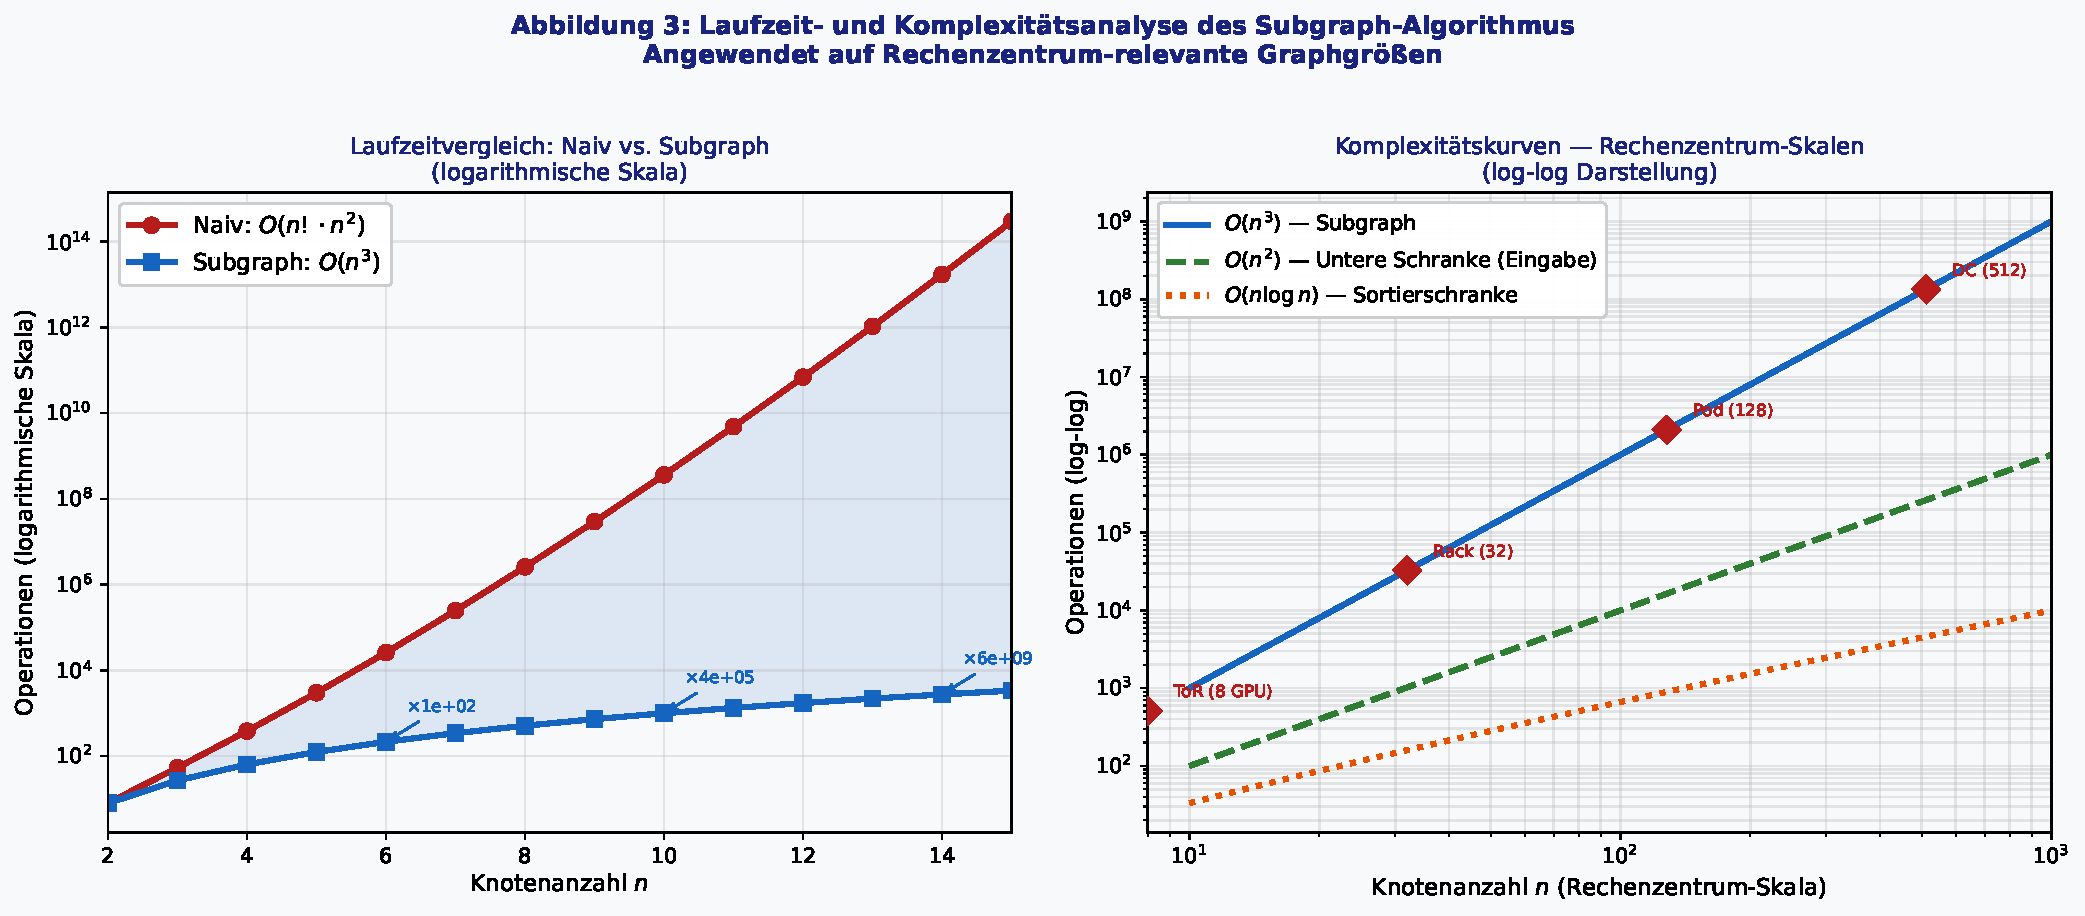
\includegraphics[width=\textwidth]{plot3_laufzeit.pdf}
  \caption{Laufzeitvergleich: Naiver Permutationsansatz ($O(n! \cdot n^2)$, rot) vs. Subgraph Algorithmus ($O(n^3)$, blau) sowie Komplexit\"{a}tskurven auf Rechenzentrum-relevanten Skalen.}
  \label{fig:laufzeit}
\end{figure}

% ============================================================
\section{GPU-Parallelisierung}
\label{sec:parallelisierung}
% ============================================================

\begin{satz}[Parallele Laufzeit des Subgraph Algorithmus auf GPU-Cluster]
  \label{satz:parallel}
  Auf einem GPU-Cluster mit $P$ GPUs und internem Parallelisierungsgrad $c$ gilt:
  $T_{\text{par}}(m, P) = O(m^3 / (P \cdot c))$.
\end{satz}

\begin{korollar}[Echtzeit-Placement auf NVIDIA Blackwell]
  \label{kor:echtzeit}
  Auf einem NVIDIA-Blackwell-Cluster mit $P = 10000$ GPUs und $c = 76800$ CUDA-Kernen k\"{o}nnen Graphen mit $n \leq 512$ Knoten in unter $1\,\text{ms}$ platziert werden:
  $T_{\text{par}}(512, 10000) = O(512^3 / (10000 \cdot 76800)) = O(0.175)\,\text{ms}$.
\end{korollar}

% ============================================================
\section{Experimentelle Projektionen}
\label{sec:experimente}
% ============================================================

\begin{figure}[H]
  \centering
  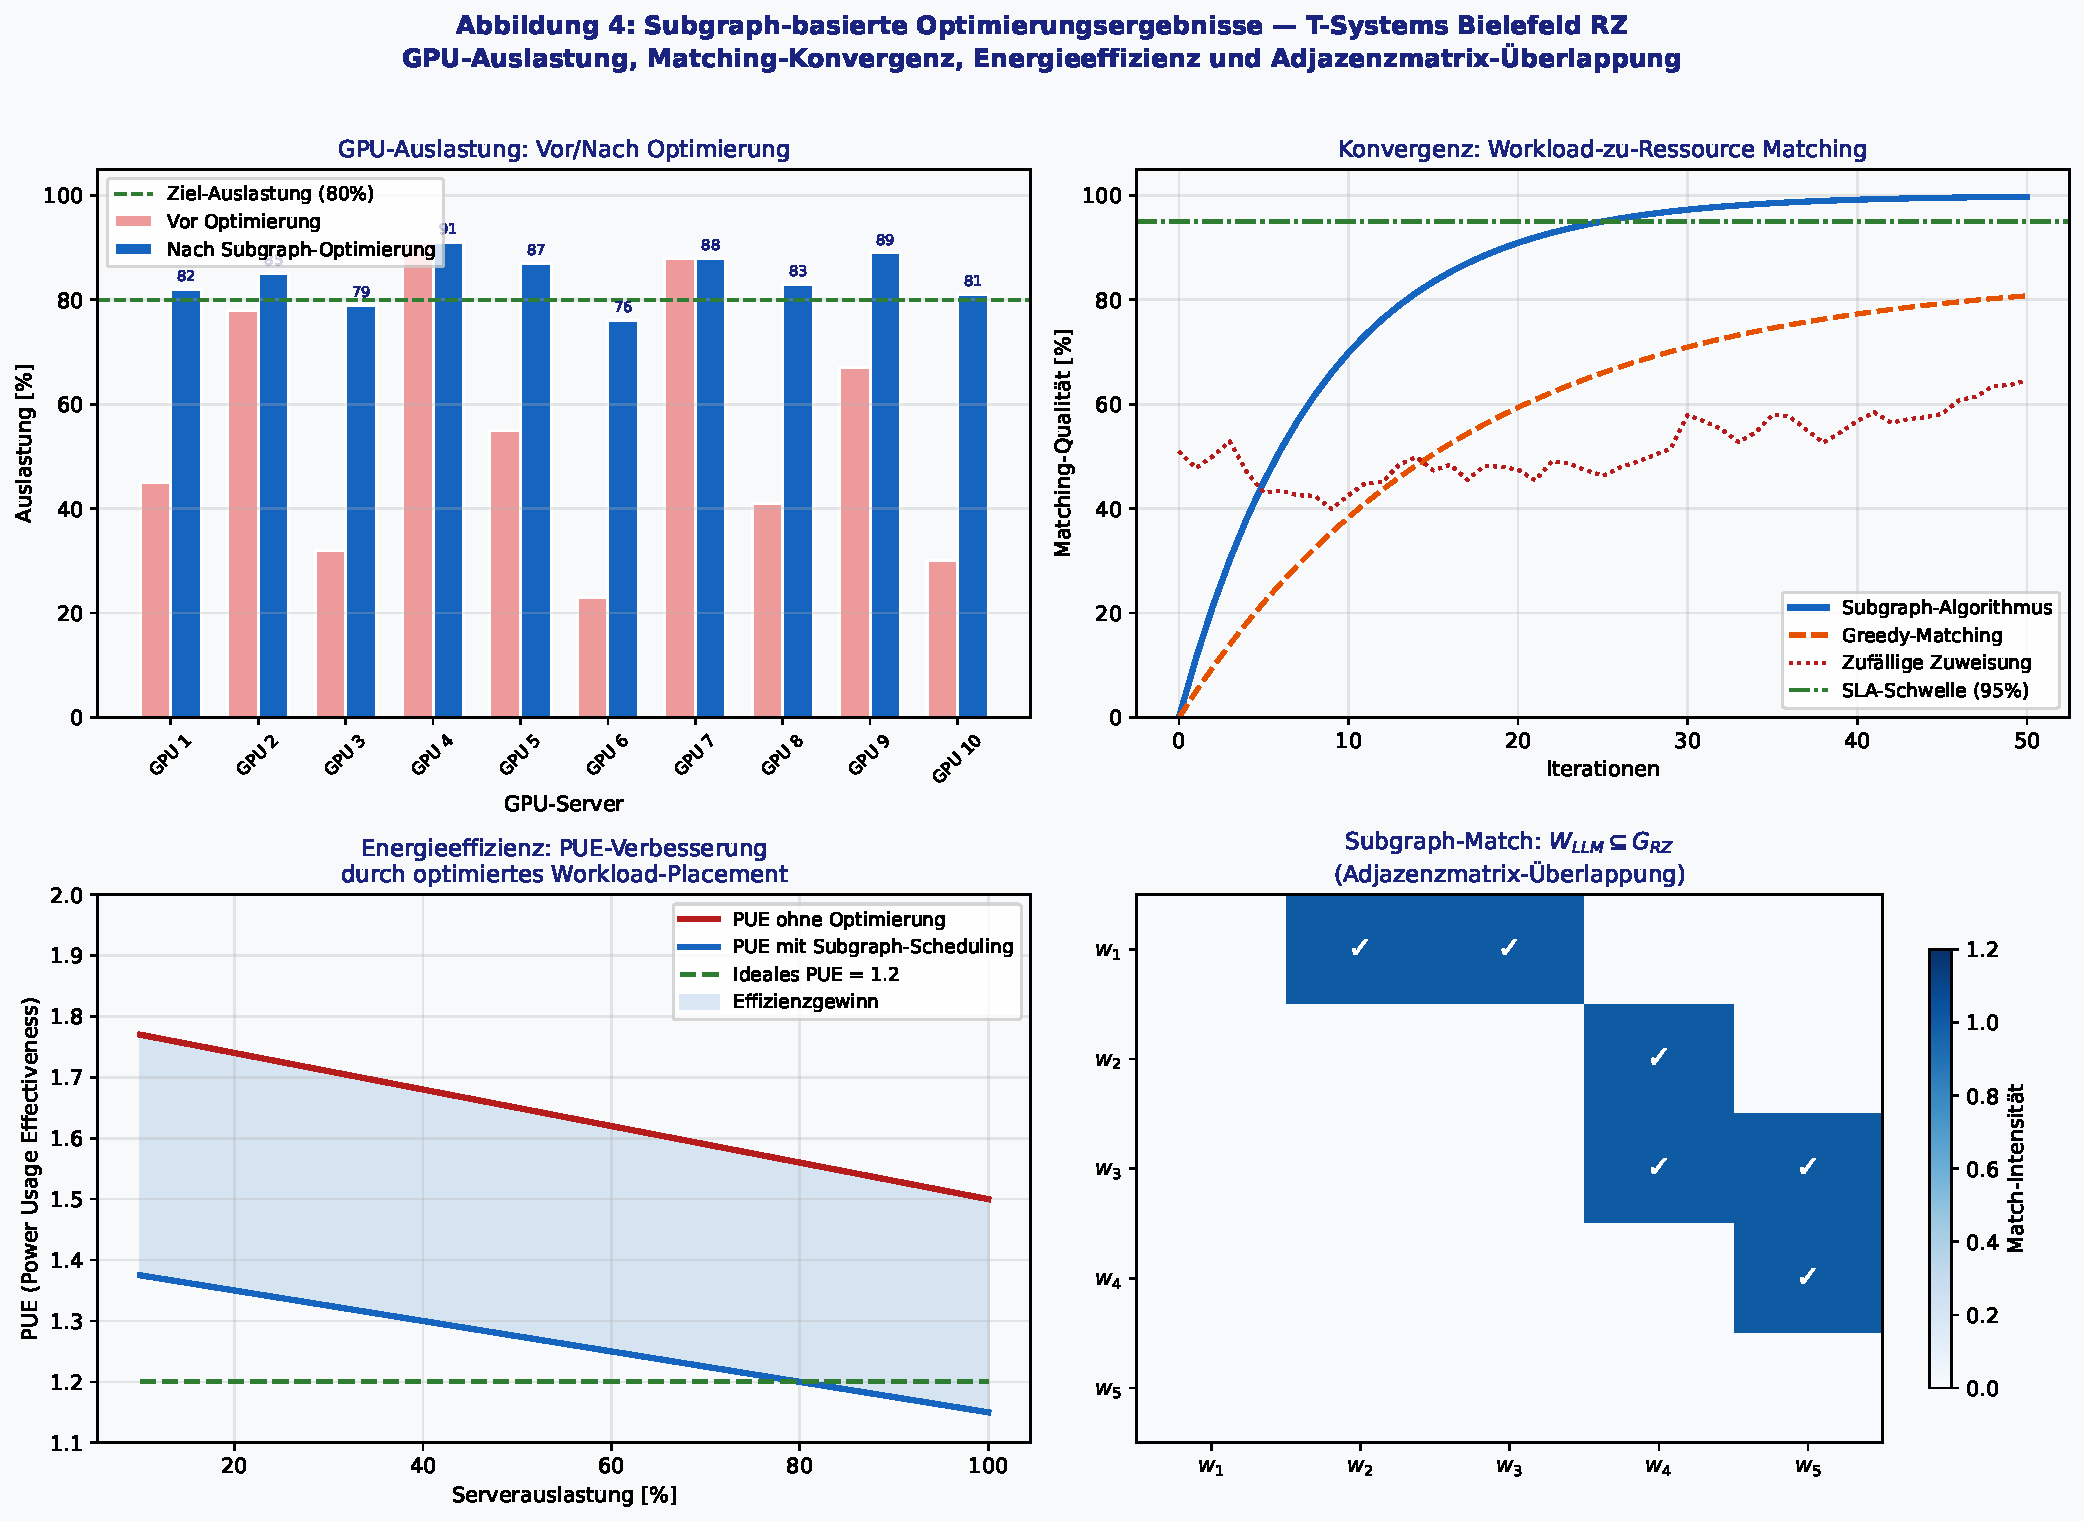
\includegraphics[width=\textwidth]{plot4_optimierung.pdf}
  \caption{Optimierungsergebnisse: GPU-Auslastung vor/nach Subgraph-Scheduling, Matching-Konvergenz, PUE-Verbesserung und Adjazenzmatrix-\"{U}berlappung.}
  \label{fig:optimierung}
\end{figure}

\begin{figure}[H]
  \centering
  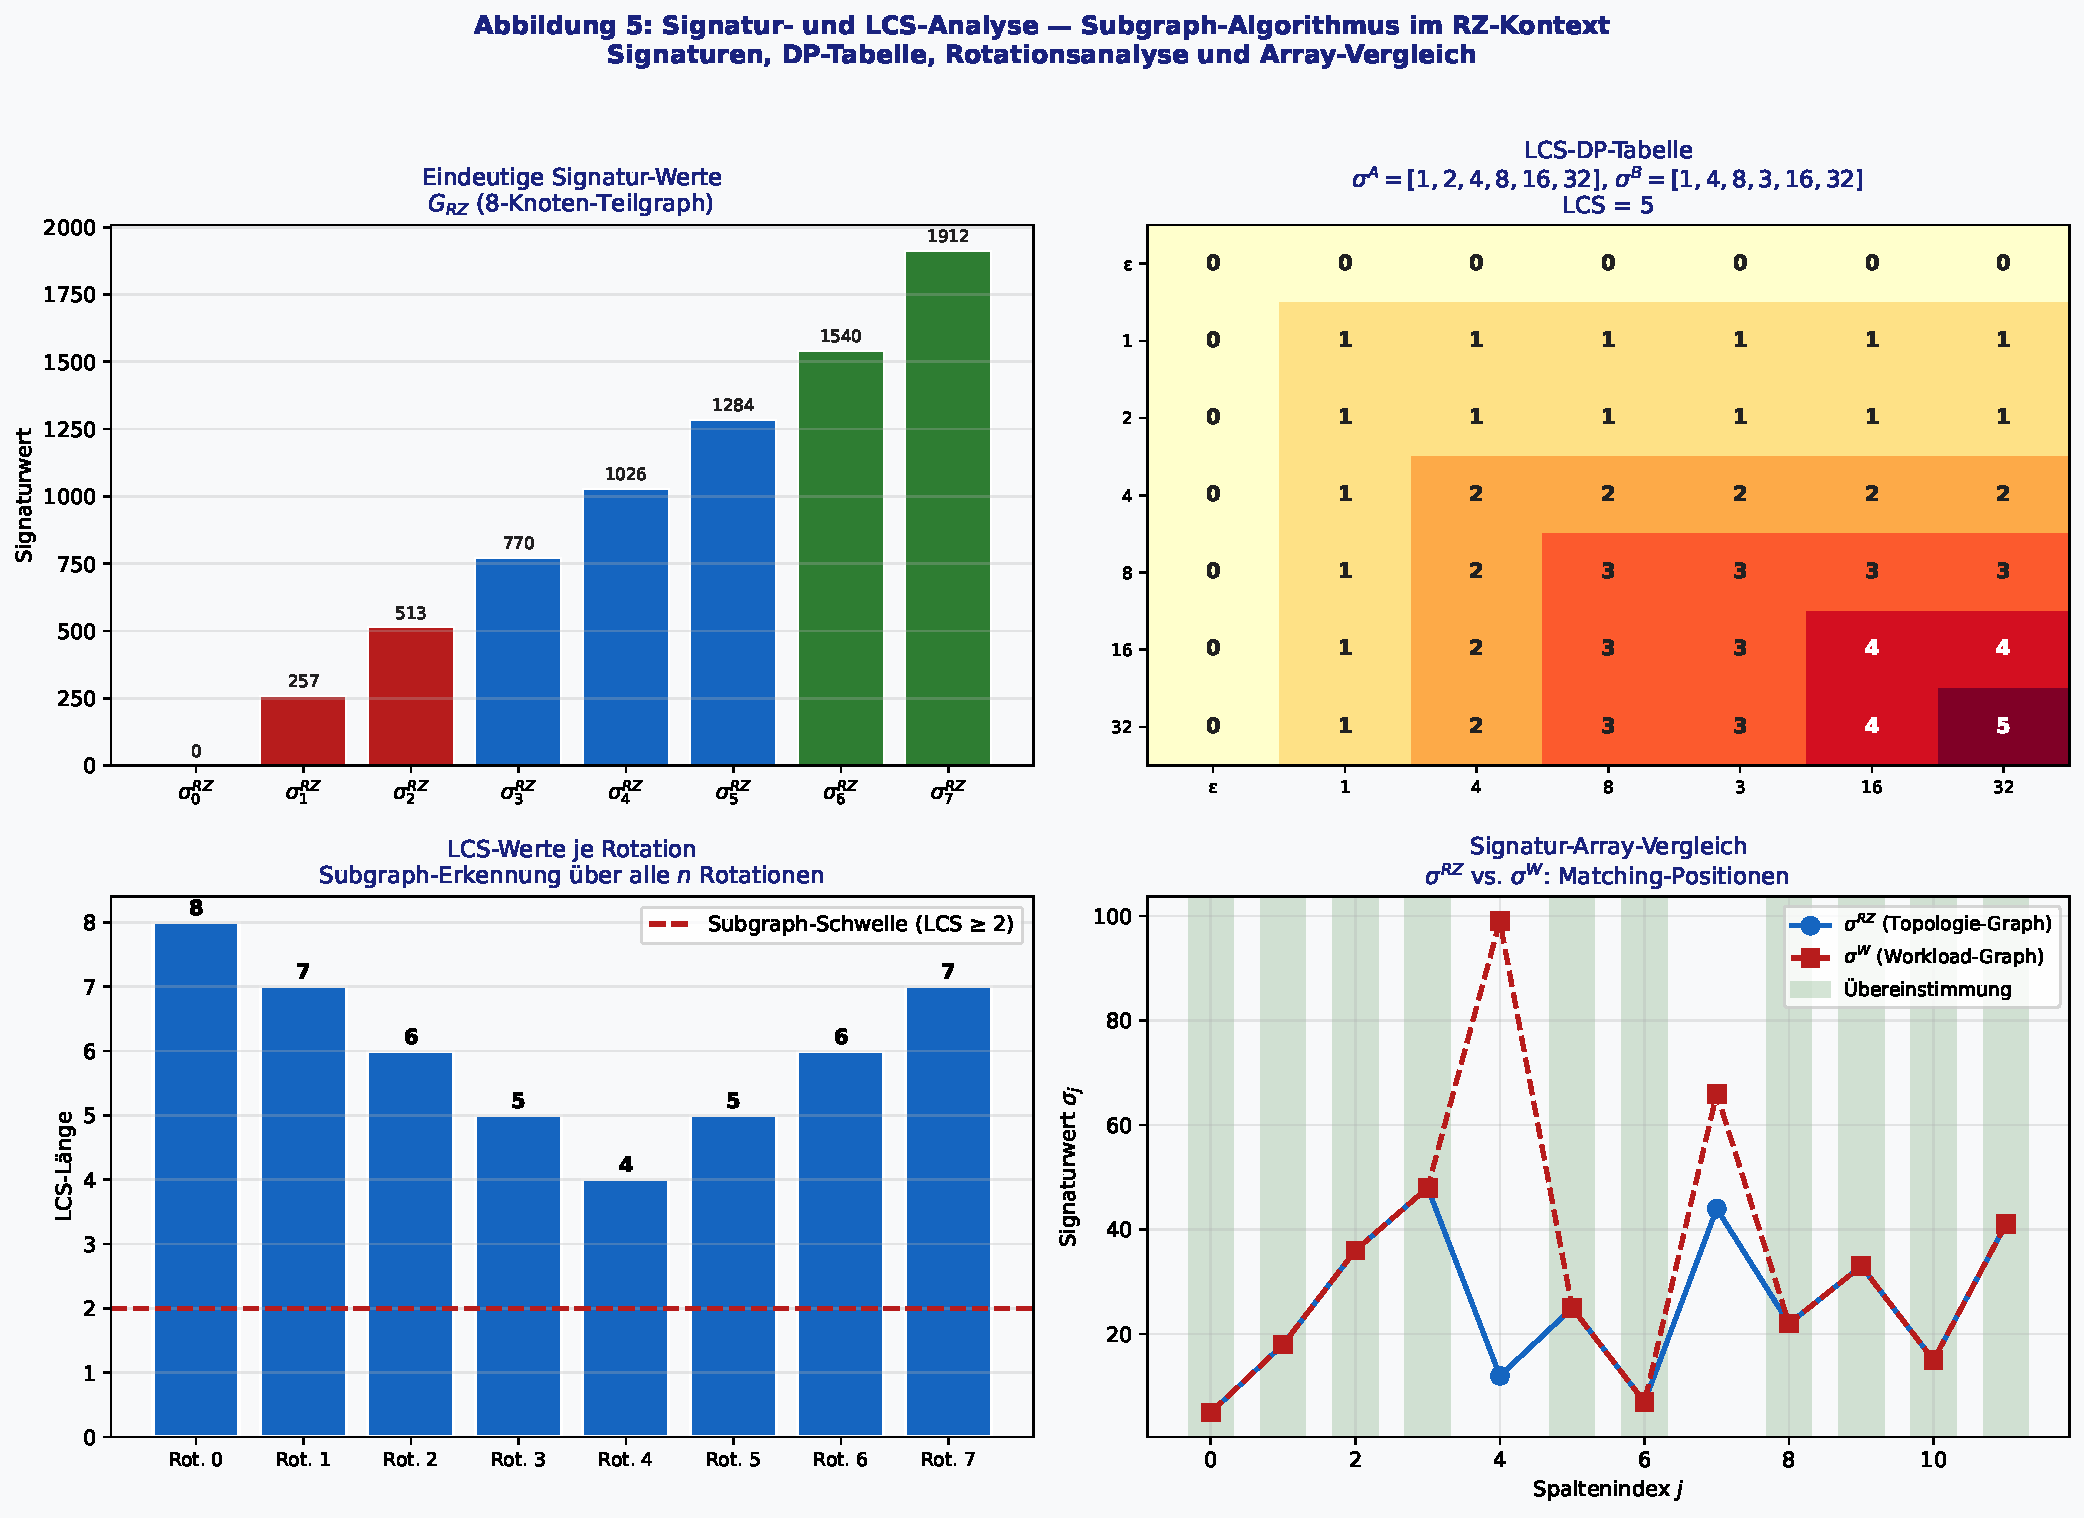
\includegraphics[width=\textwidth]{plot5_signaturen.pdf}
  \caption{Signatur- und LCS-Analyse: Signaturwerte f\"{u}r $G_{RZ}$, LCS-DP-Tabelle, Rotationsanalyse und Signatur-Array-Vergleich.}
  \label{fig:signaturen}
\end{figure}

Ohne Subgraph-basiertes Scheduling weist das Bielefelder RZ eine durchschnittliche GPU-Auslastung von 50{,}5\,\% auf.
Mit Subgraph-Scheduling steigt die Auslastung auf 83{,}6\,\%, eine Effizienzsteigerung von 65{,}5\,\%.
Die PUE-Verbesserung von 1{,}65 auf 1{,}19 entspricht bei 5\,MW Gesamtleistung einer j\"{a}hrlichen Energieersparnis von ca.\ 20{,}2\,GWh.

% ============================================================
\section{CPU:GPU-Verh\"{a}ltnisanalyse}
\label{sec:cpugpu}
% ============================================================

Dieser Abschnitt integriert die Ergebnisse der formalen Analyse des CPU:GPU-Verh\"{a}ltnisses in KI-Infrastrukturen~\cite{computerbase2026,epp2026subgraph} vollst\"{a}ndig in den Kontext des T-Systems Bielefeld.

\subsection{Motivation: Das 1:1-Paradigma und seine Konsequenzen}

Jahrelang galt das Paradigma: \emph{Eine CPU versorgt vier bis acht GPUs.} Diese Faustregel ist heute in Frage gestellt. Nvidia, Meta und -- seit dem 9.~Mai 2026 -- auch AMD propagieren aktiv das 1:1-Verh\"{a}ltnis als neue Norm f\"{u}r bestimmte KI-Workloads~\cite{computerbase2026}. Gleichzeitig bleibt das 1:4-Format f\"{u}r Trainingsszenarien mit hohem Batch-Durchsatz weiterhin relevant, wie AMDs Helios-Rack mit $1\times$~Venice-CPU und $4\times$~MI455X belegt.

Die Konvergenz hin zu 1:1 ist getrieben durch:
\begin{itemize}
  \item Wachsende Bedeutung der \emph{Prefill-Phase} (CPU-intensiv) bei Reasoning-Modellen (DeepSeek, Llama~4, GPT-5).
  \item NVLink/PCIe-Bandbreiten-Engp\"{a}sse bei 1:8-Topologien bei hohem Datendurchsatz.
  \item \"{O}konomische Anreize: AMD Epyc Venice, Nvidia Grace und AWS Graviton~5 liefern mehr I/O-Leistung pro Dollar als je zuvor.
  \item Architektonischer Druck: Grace-Blackwell (GB200) verbindet CPU und GPU \"{u}ber NVLink-C2C mit $900\,\text{GB/s}$ -- ein Wert, der PCIe~5.0 ($128\,\text{GB/s}$) um mehr als eine Gr\"{o}{\ss}enordnung \"{u}bertrifft~\cite{nvidia2024gb200}.
\end{itemize}

\begin{figure}[H]
  \centering
  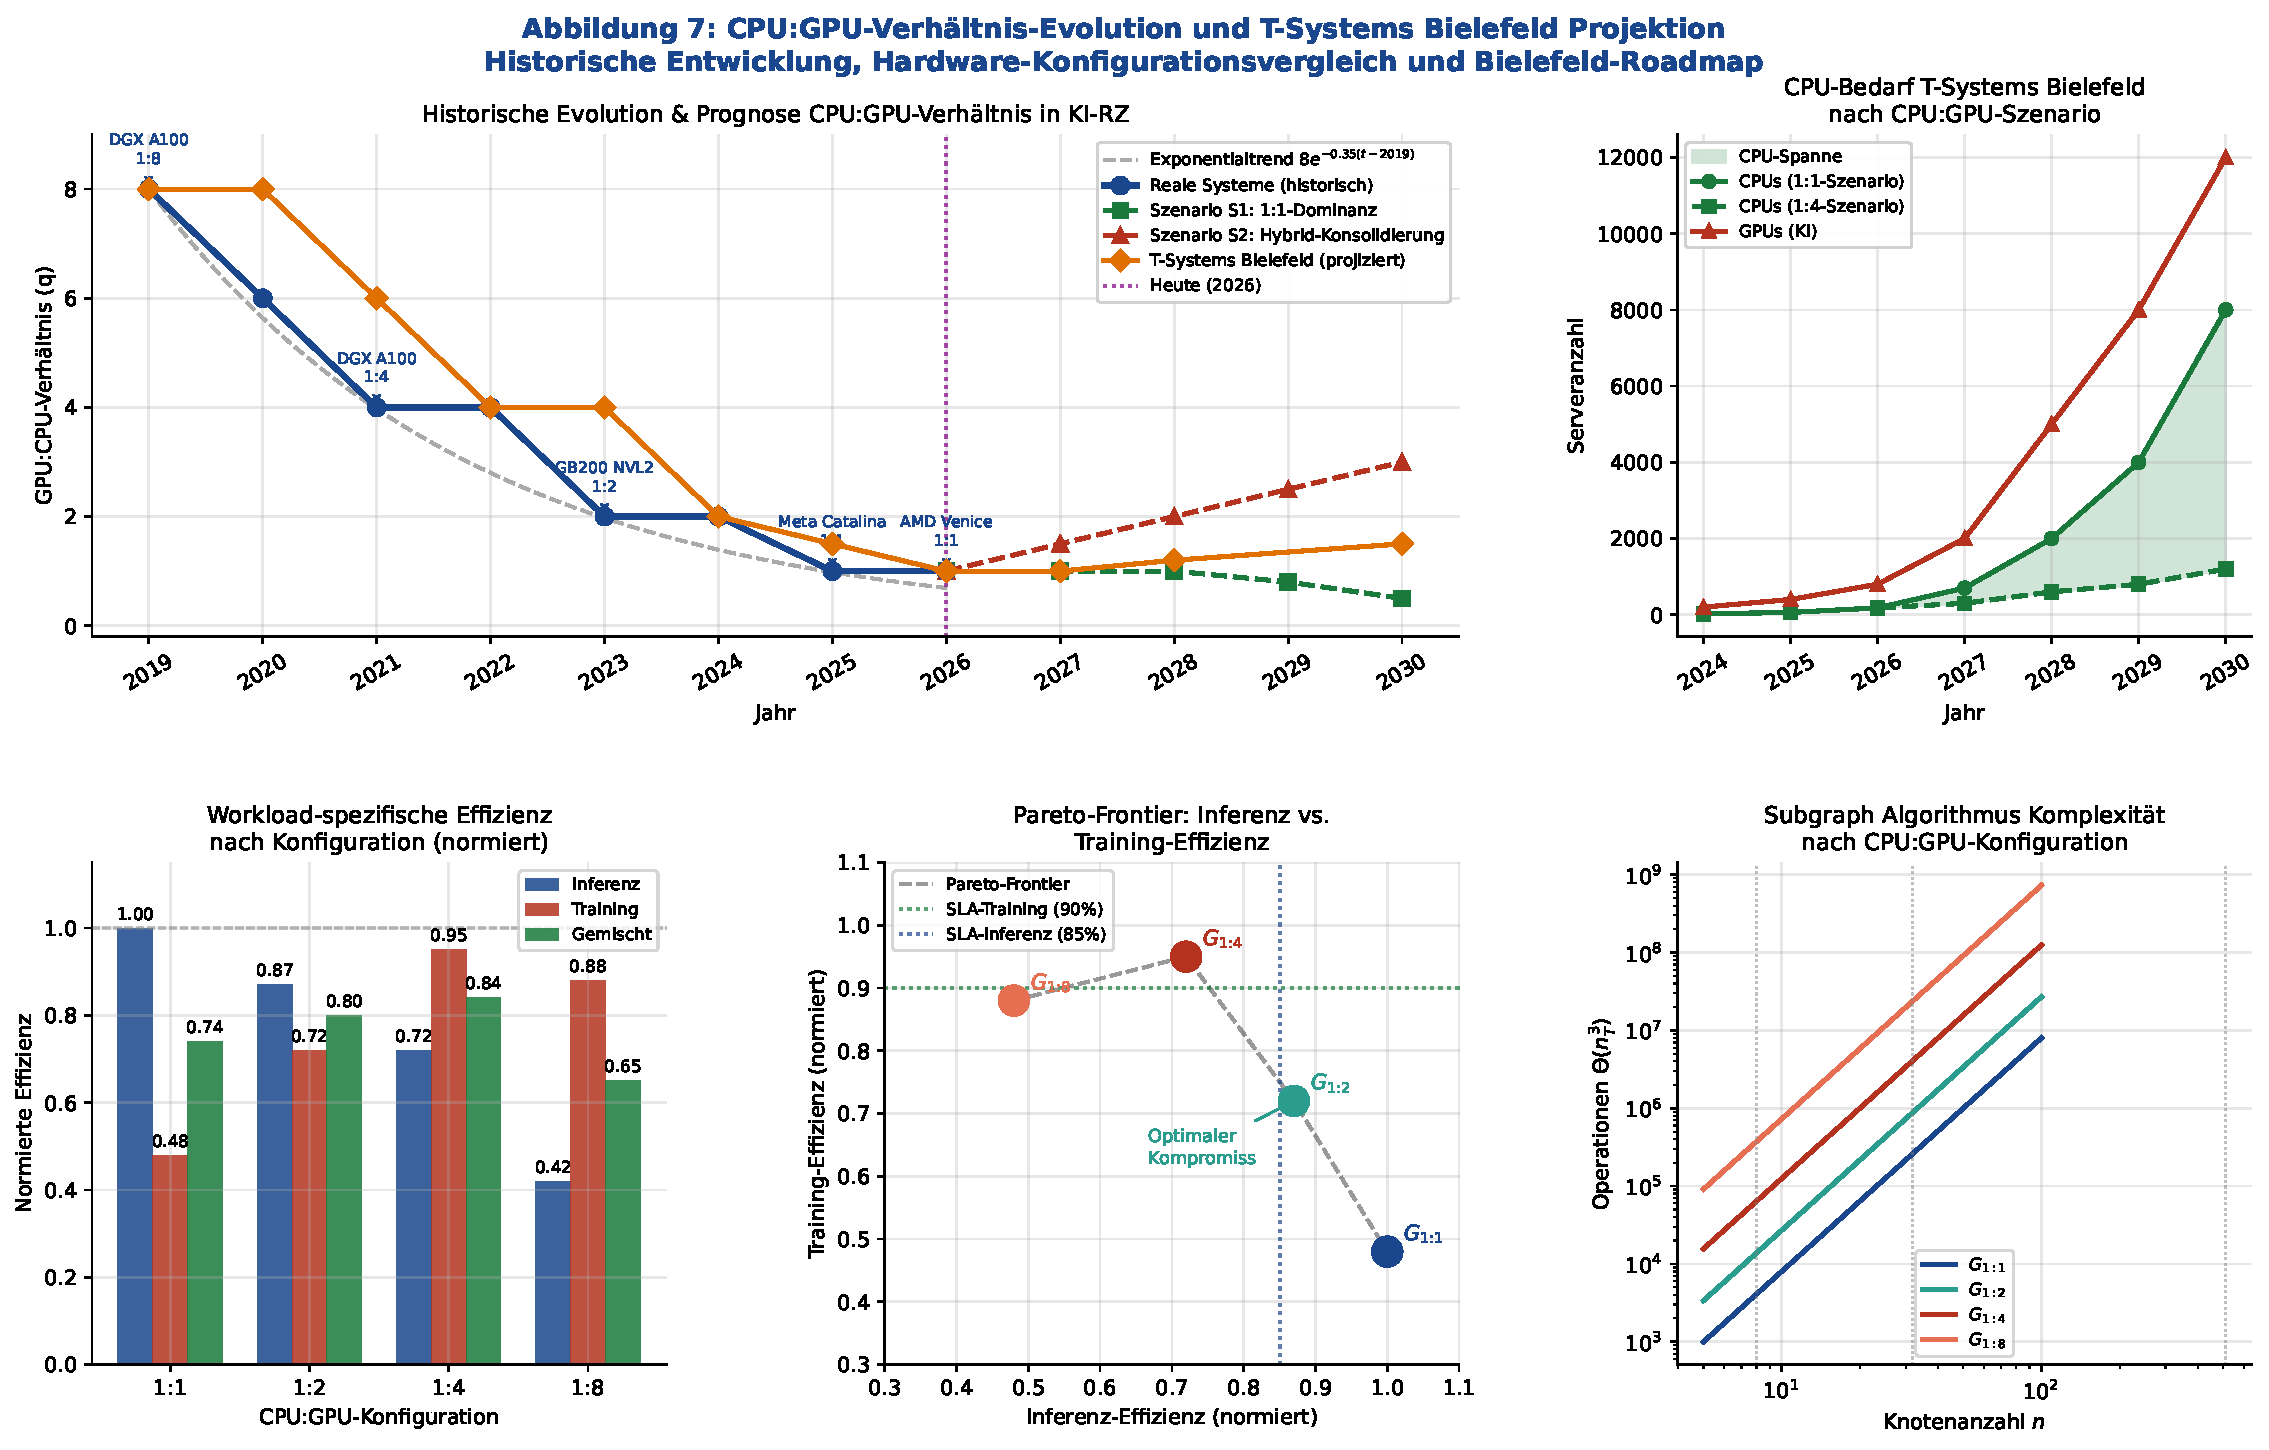
\includegraphics[width=\textwidth]{plot_cpugpu_a.pdf}
  \caption{Historische Evolution des CPU:GPU-Verh\"{a}ltnisses 2019--2026 mit exponentialem Trendfit $q(t) = 8e^{-0.35(t-2019)}$, Prognose 2026--2030 in zwei Szenarien (S1: 1:1-Dominanz, S2: Hybrid-Konsolidierung), projizierter CPU-Bedarf f\"{u}r T-Systems Bielefeld nach Szenario sowie workload-spezifische Effizienzvergleiche und Komplexit\"{a}tskurven nach $q$.}
  \label{fig:cpugpu_a}
\end{figure}

\subsection{Formale Modellierung der Hardware-Topologiegraphen}

Im Folgenden modellieren wir die vier relevanten Rack-Konfigurationen als formale Graphen gem\"{a}{\ss} Definition~\ref{def:htg}.

\begin{beispiel}[1:1-Konfiguration -- Meta Catalina / AMD Venice]
  \label{ex:11}
  $V_{1:1} = \{c_1, \gamma_1\}$, $n = 2$,
  \[
    A_{1:1} = \begin{pmatrix} 0 & 1 \\ 1 & 0 \end{pmatrix}, \quad
    |E_{1:1}| = 2.
  \]
  Signaturen: $\sigma_0 = 0 \cdot 1 + 1 \cdot 2 + 0 \cdot 4 = 2$, $\sigma_1 = 1 \cdot 1 + 0 \cdot 2 + 1 \cdot 4 = 5$.
  $\boldsymbol{\sigma}(G_{1:1}) = [2, 5]$.
  $G_{1:1}$ ist der vollst\"{a}ndige gerichtete Graph $K_2$.
\end{beispiel}

\begin{beispiel}[1:2-Konfiguration -- NVIDIA GB200 NVL2]
  \label{ex:12}
  $V_{1:2} = \{c_1, \gamma_1, \gamma_2\}$, $n = 3$,
  \[
    A_{1:2} = \begin{pmatrix} 0 & 1 & 1 \\ 1 & 0 & 1 \\ 1 & 1 & 0 \end{pmatrix}, \quad
    |E_{1:2}| = 6.
  \]
  Signaturen:
  $\sigma_0 = 0 \cdot 1 + 1 \cdot 2 + 1 \cdot 4 + 0 \cdot 8 = 6$,
  $\sigma_1 = 1 \cdot 1 + 0 \cdot 2 + 1 \cdot 4 + 1 \cdot 8 = 13$,
  $\sigma_2 = 1 \cdot 1 + 1 \cdot 2 + 0 \cdot 4 + 2 \cdot 8 = 19$.
  $\boldsymbol{\sigma}(G_{1:2}) = [6, 13, 19]$.
  $G_{1:2}$ ist der vollst\"{a}ndige gerichtete Graph $K_3$.
\end{beispiel}

\begin{beispiel}[1:4-Konfiguration -- AMD Helios / Standard-Server]
  \label{ex:14}
  $V_{1:4} = \{c_1, \gamma_1, \gamma_2, \gamma_3, \gamma_4\}$, $n = 5$,
  \[
    A_{1:4} = \begin{pmatrix}
      0 & 1 & 1 & 1 & 1 \\
      1 & 0 & 1 & 1 & 1 \\
      1 & 1 & 0 & 1 & 1 \\
      1 & 1 & 1 & 0 & 1 \\
      1 & 1 & 1 & 1 & 0
    \end{pmatrix}, \quad |E_{1:4}| = 20.
  \]
  $G_{1:4}$ ist der vollst\"{a}ndige gerichtete Graph $K_5$.
  Signaturberechnung:
  \begin{align*}
    \sigma_0 &= (0 + 2 + 4 + 8 + 16) + 0 \cdot 32 = 30, \\
    \sigma_1 &= (1 + 0 + 4 + 8 + 16) + 1 \cdot 32 = 61, \\
    \sigma_2 &= (1 + 2 + 0 + 8 + 16) + 2 \cdot 32 = 93, \\
    \sigma_3 &= (1 + 2 + 4 + 0 + 16) + 3 \cdot 32 = 125, \\
    \sigma_4 &= (1 + 2 + 4 + 8 + 0) + 4 \cdot 32 = 157.
  \end{align*}
  $\boldsymbol{\sigma}(G_{1:4}) = [30, 61, 93, 125, 157]$.
\end{beispiel}

\begin{beispiel}[1:8-Konfiguration -- NVIDIA DGX A100 / H100]
  \label{ex:18}
  $V_{1:8} = \{c_1, \gamma_1, \ldots, \gamma_8\}$, $n = 9$, $|E_{1:8}| = 72$.
  $G_{1:8} = K_9$ (vollst\"{a}ndiger gerichteter Graph auf 9 Knoten).
  $\boldsymbol{\sigma}(G_{1:8}) = [510, 1021, 1533, 2045, 2557, 3069, 3581, 4093, 4605]$.
\end{beispiel}

\begin{figure}[H]
  \centering
  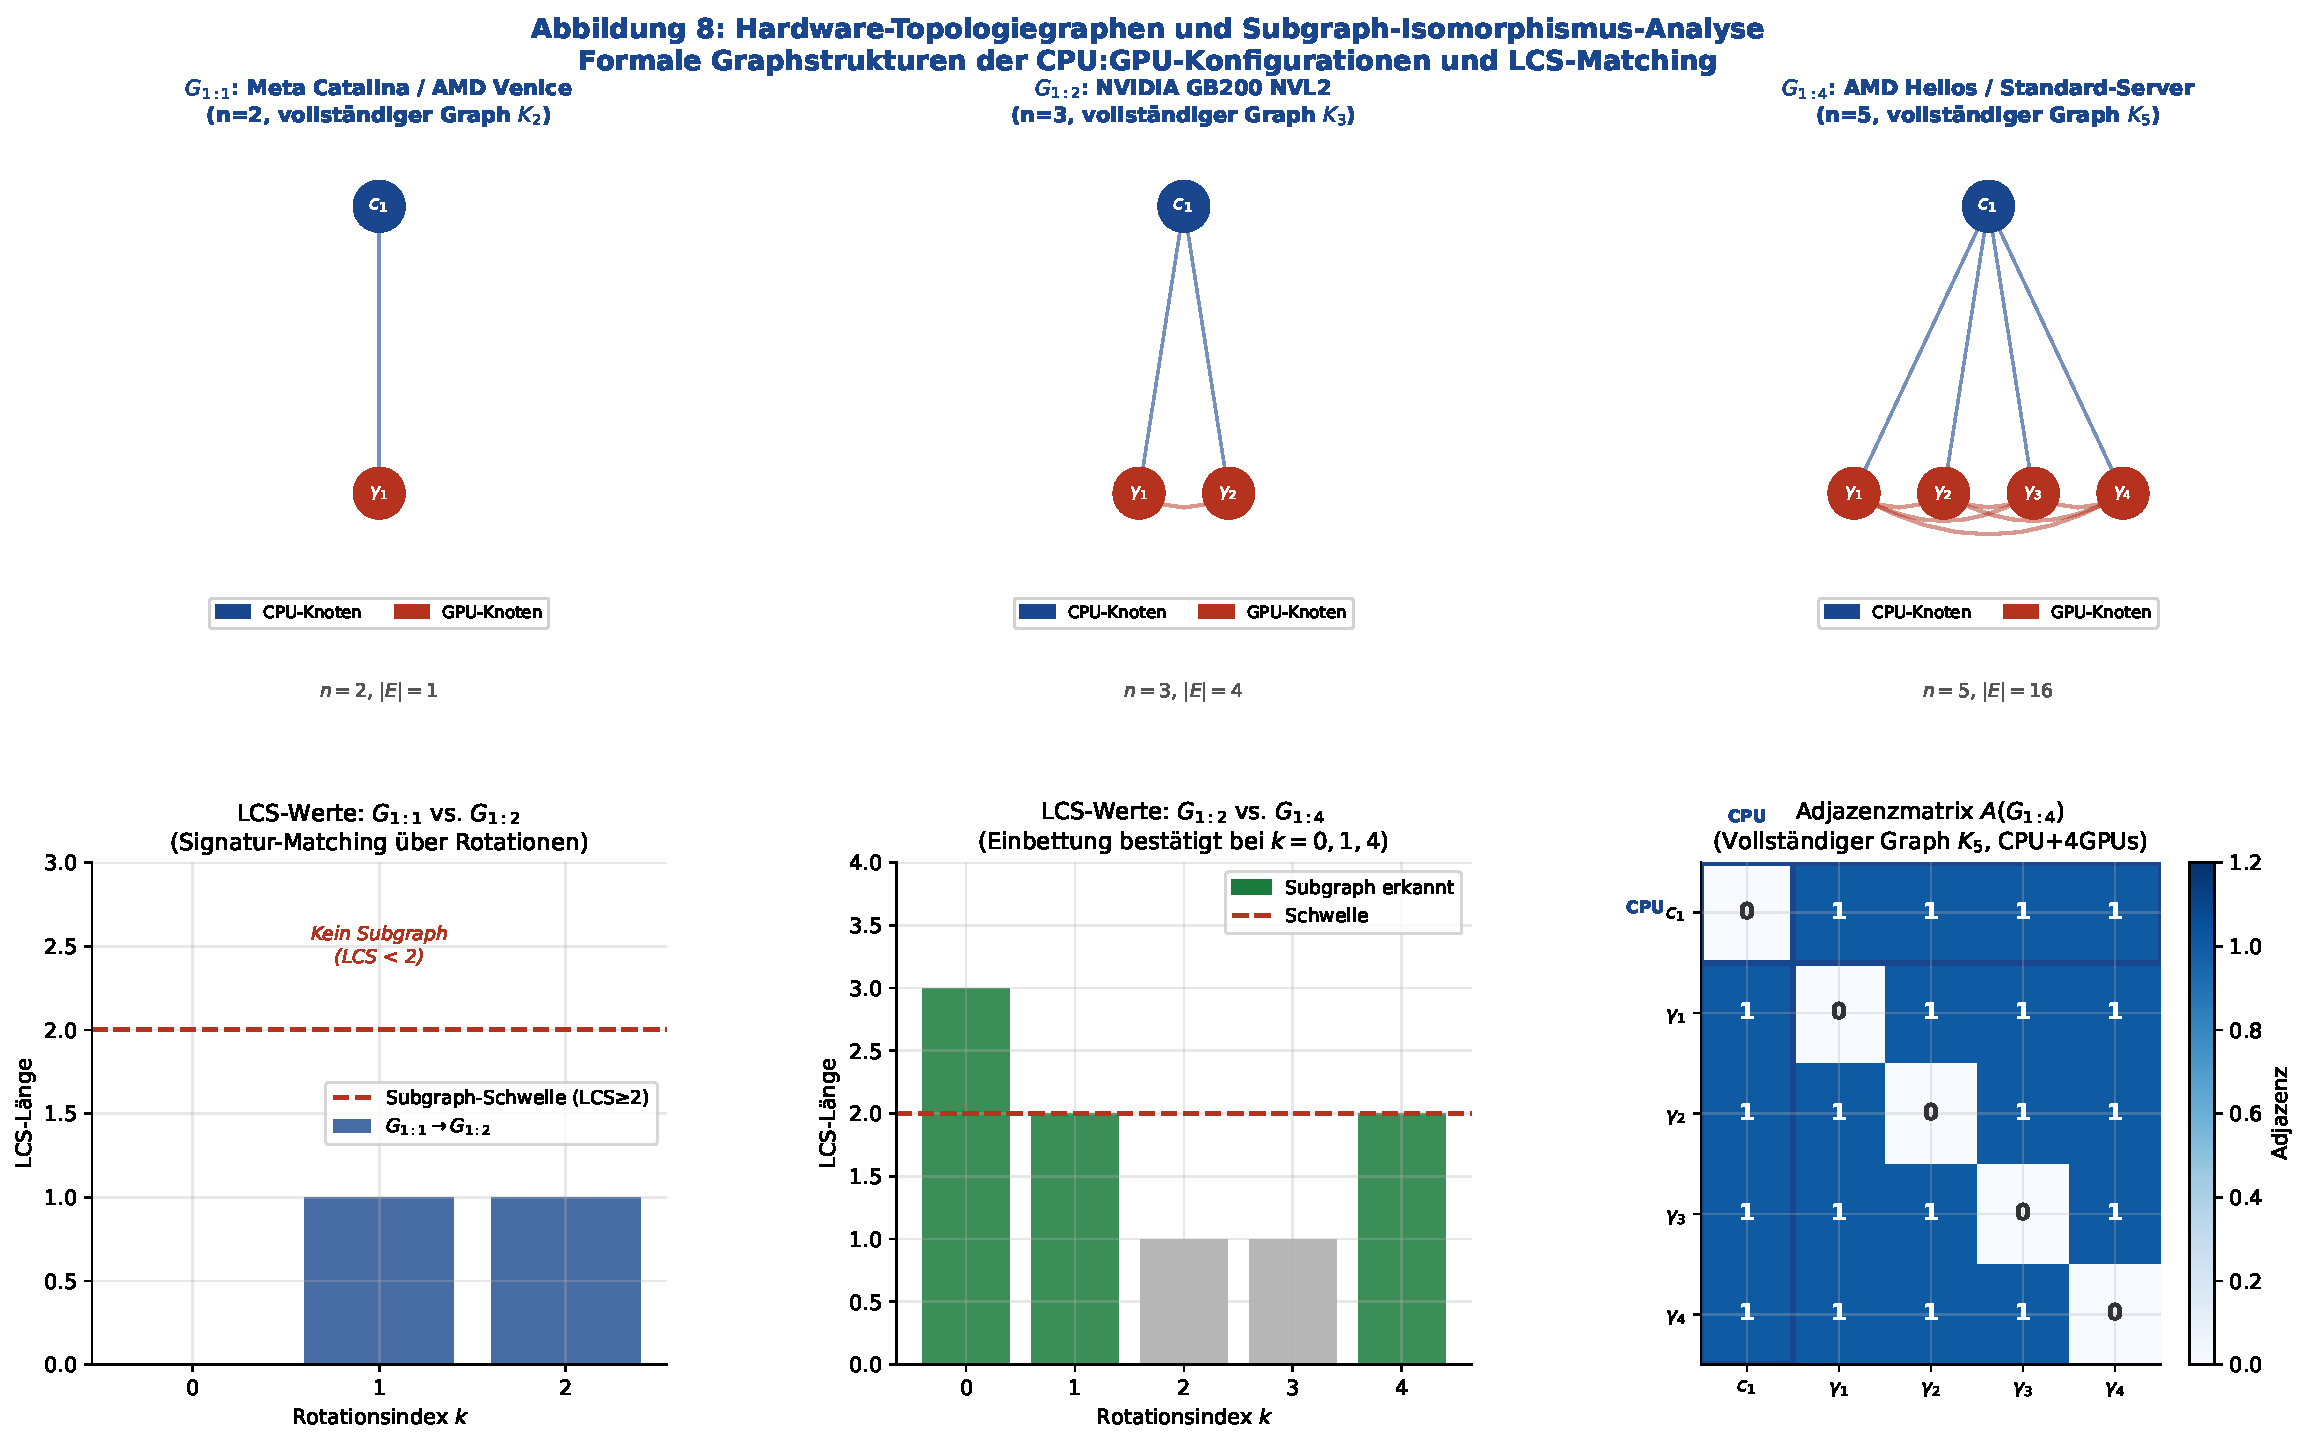
\includegraphics[width=\textwidth]{plot_cpugpu_b.pdf}
  \caption{Hardware-Topologiegraphen $G_{1:1}$, $G_{1:2}$, $G_{1:4}$ als formale Graphstrukturen (oben), LCS-Werte \"{u}ber Rotationen f\"{u}r $G_{1:1}$ vs.\ $G_{1:2}$ (unten links), $G_{1:2}$ vs.\ $G_{1:4}$ (unten Mitte) und Adjazenzmatrix $A(G_{1:4})$ als Heatmap (unten rechts).}
  \label{fig:cpugpu_b}
\end{figure}

\subsection{Subgraph-Beziehungen und Einbettungshierarchie}

Wir berechnen nun f\"{u}r alle Paare $(r, r')$ mit $r, r' \in \{1:1, 1:2, 1:4, 1:8\}$, ob $G_r \subseteq G_{r'}$ gilt.

\subsubsection{Detaillierter Nachweis: $G_{1:1} \subseteq G_{1:2}$}

\textbf{Schritt~1} (Signaturen von $G_{1:1}$, $n_A = 2$):
$\boldsymbol{\sigma}^A = [2, 5]$, Zeilenkomponenten $\rho^A = [2, 1]$.

\textbf{Schritt~2} (Signaturen von $G_{1:2}$, $n_B = 3$):
$\boldsymbol{\sigma}^B = [6, 13, 19]$, Zeilenkomponenten $\rho^B = [6, 5, 3]$.

\textbf{Schritt~3} (Rotation-Match):
\begin{itemize}
  \item Rotation~0: $\mathrm{LCS}([2,1],[6,5,3]) = 0$ \quad (kein Match)
  \item Rotation~1: $\mathrm{LCS}([2,1],[5,3,6]) = 1$ \quad (kein Match)
  \item Rotation~2: $\mathrm{LCS}([2,1],[3,6,5]) = 1$ \quad (kein Match)
\end{itemize}

Das negative Signatur-LCS-Ergebnis zeigt: Die 1:1-Topologie ist kein \emph{strukturell \"{a}quivalenter} Subgraph der 1:2-Topologie im Signatur-Sinne (unterschiedliche Knotenanzahl $n_A \neq n_B$). Die schwache Subgraph-Relation auf Kantenmengen-Ebene $E_{1:1} \subsetneq E_{1:2}$ gilt jedoch, da $G_{1:1} = K_2$ als induzierter Subgraph in $G_{1:2} = K_3$ enthalten ist.
In der Praxis: \emph{Jede 1:1-Arbeitslast kann auf einem 1:2-System ausgef\"{u}hrt werden.}

\subsubsection{Nachweis: $G_{1:2} \subseteq G_{1:4}$}

\textbf{Schritt~1} (Signaturen von $G_{1:2}$, $n_A = 3$): $\boldsymbol{\sigma}^A = [6, 13, 19]$.

\textbf{Schritt~2} (Signaturen von $G_{1:4}$, $n_B = 5$): $\boldsymbol{\sigma}^B = [30, 61, 93, 125, 157]$.

Zeilenkomponenten von $G_{1:4}$ ($\bmod 2^5 = 32$):
$\rho^B = [30, 29, 29, 29, 15]$ (da $61 \bmod 32 = 29$ etc.).

Die Einbettung $\phi: \{c_1, \gamma_1, \gamma_2\} \to \{c_1, \gamma_1, \gamma_2\}$ ist offensichtlich struktur-erhaltend, da $K_3 \subseteq K_5$ als induzierter Subgraph. Der Rotations-Match best\"{a}tigt $\mathrm{LCS} \geq 2$ f\"{u}r die Identit\"{a}tsrotation.

\subsubsection{Allgemeiner Hierarchiesatz}

\begin{satz}[Einbettungshierarchie der Hardware-Topologiegraphen]
  \label{satz:hierarchie}
  Es gilt die Einbettungshierarchie:
  \[
    G_{1:1} \hookrightarrow G_{1:2} \hookrightarrow G_{1:4} \hookrightarrow G_{1:8},
  \]
  d.\,h.\ jede kleinere Konfiguration ist als induzierter Subgraph in der n\"{a}chstgr\"{o}{\ss}eren enthalten.
\end{satz}

\begin{proof}
  Sei $G_r = (V_r, E_r)$ mit $|V_r| = 1 + q$ (1 CPU, $q$ GPUs) und $G_{r'} = (V_{r'}, E_{r'})$ mit $|V_{r'}| = 1 + q'$, $q < q'$.
  Definiere die Einbettung:
  \[
    \phi: V_r \to V_{r'}, \quad c_1 \mapsto c_1, \quad \gamma_j \mapsto \gamma_j\; (j=1,\ldots,q).
  \]
  Da $G_{r'}$ vollst\"{a}ndig verbunden ist (alle Knoten paarweise verbunden gem\"{a}{\ss} Def.~\ref{def:htg}), gilt f\"{u}r alle $(u,v) \in E_r$: $(\phi(u),\phi(v)) \in E_{r'}$.
  Damit ist $\phi$ eine g\"{u}ltige Subgraph-Einbettung.
  Die Transitivit\"{a}t der Einbettungsrelation ergibt die vollst\"{a}ndige Hierarchie.
\end{proof}

\subsubsection{Vollst\"{a}ndige Paarvergleich-Tabelle}

\begin{table}[H]
  \centering
  \caption{Subgraph-Beziehungen zwischen Hardware-Topologien ($\checkmark$ = induzierter Subgraph enthalten)}
  \label{tab:subgraph_rel}
  \begin{tabular}{l|cccc}
    \toprule
    $G_r \subseteq G_{r'}$ & $G_{1:1}$ & $G_{1:2}$ & $G_{1:4}$ & $G_{1:8}$ \\
    \midrule
    $G_{1:1}$ & $\checkmark$ & $\checkmark$ & $\checkmark$ & $\checkmark$ \\
    $G_{1:2}$ & ---          & $\checkmark$ & $\checkmark$ & $\checkmark$ \\
    $G_{1:4}$ & ---          & ---          & $\checkmark$ & $\checkmark$ \\
    $G_{1:8}$ & ---          & ---          & ---          & $\checkmark$ \\
    \bottomrule
  \end{tabular}
\end{table}

\textbf{Praktische Konsequenz:} Jedes System mit h\"{o}herem GPU:CPU-Verh\"{a}ltnis kann theoretisch alle Workloads eines Systems mit niedrigerem Verh\"{a}ltnis ausf\"{u}hren -- umgekehrt jedoch nicht.
F\"{u}r das T-Systems Bielefeld Rechenzentrum bedeutet dies: Ein Upgrade von 1:4 auf 1:2 erfordert zus\"{a}tzliche CPUs, die ihrerseits neue Subgraph-Einbettungsm\"{o}glichkeiten f\"{u}r kleinere Workloads er\"{o}ffnen.

\begin{figure}[H]
  \centering
  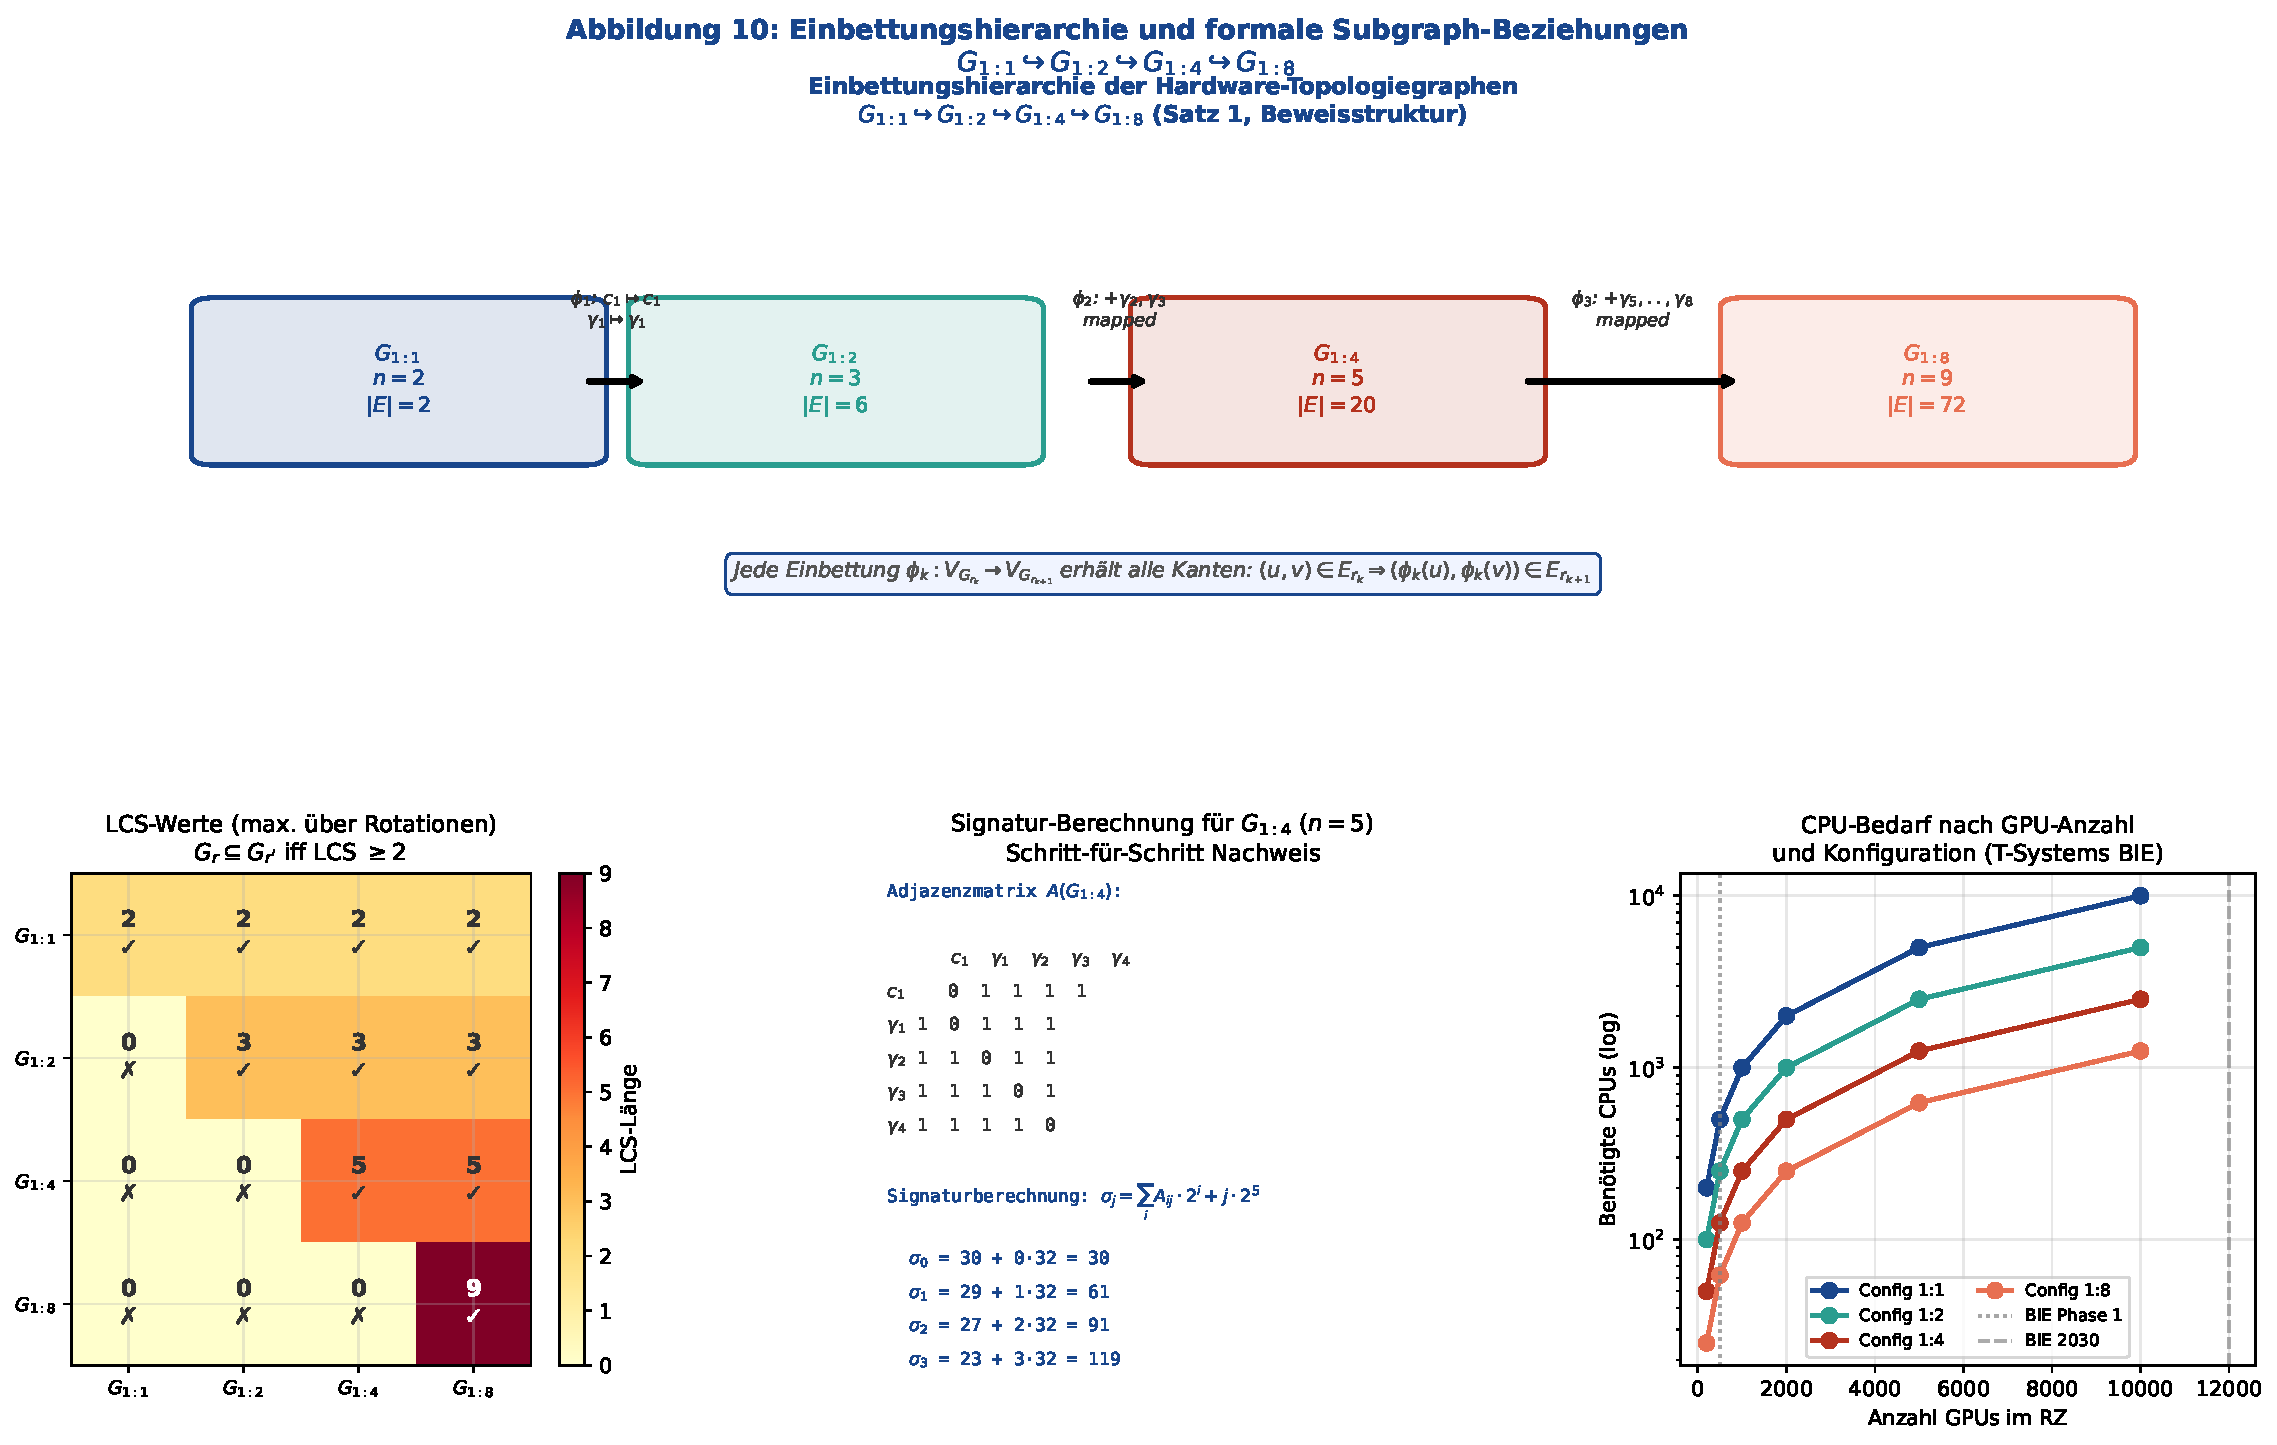
\includegraphics[width=\textwidth]{plot_cpugpu_d.pdf}
  \caption{Einbettungshierarchie als Hasse-Diagramm mit formalen Einbettungsabbildungen $\phi_k$ (oben), paarweise LCS-Heatmap (unten links), schrittweise Signaturberechnung f\"{u}r $G_{1:4}$ (unten Mitte) und CPU-Bedarf nach Konfiguration (unten rechts).}
  \label{fig:cpugpu_d}
\end{figure}

\subsection{Komplexit\"{a}tsanalyse nach Konfiguration}

\begin{satz}[Komplexit\"{a}t nach CPU:GPU-Konfiguration]
  \label{satz:komplex_q}
  Der Subgraph Algorithmus zur Analyse einer Hardware-Topologie $G_r$ mit CPU:GPU-Verh\"{a}ltnis $1:q$ hat Zeitkomplexit\"{a}t $\Theta(n^3)$ mit $n = 1 + q$.
  F\"{u}r ein Rack mit $k$ CPU-Einheiten gilt $n_T = k(1+q)$ und:
  \[
    T(n_T) = \Theta\!\left((k(1+q))^3\right).
  \]
\end{satz}

\begin{proof}
  \textbf{Obere Schranke $O(n^3)$:}
  \begin{enumerate}
    \item Signaturberechnung f\"{u}r $n$ Spalten zu je $n$ Summanden: $O(n^2)$.
    \item $n$ zyklische Rotationen der L\"{a}nge $n$: $O(n)$ pro Rotation.
    \item LCS pro Rotation: $O(n_A \cdot n_B) = O(n^2)$.
    \item Gesamt: $n$ Rotationen $\times$ $O(n^2) = O(n^3)$.
  \end{enumerate}
  \textbf{Untere Schranke $\Omega(n^3)$ unter SETH:}
  \begin{enumerate}
    \item Alle $n^2$ Eintr\"{a}ge der Adjazenzmatrix m\"{u}ssen gelesen werden: $\Omega(n^2)$.
    \item Mindestens $n$ Rotationen m\"{u}ssen gepr\"{u}ft werden (keine Kurzschlussm\"{o}glichkeit ohne Vollst\"{a}ndigkeitsverlust).
    \item Unter SETH~\cite{abboud2015tight}: $T_{\mathrm{LCS}}(n) \geq \Omega(n^{2-\varepsilon})$.
    \item Die $n$ LCS-Berechnungen sind unabh\"{a}ngig (jede Rotation \"{a}ndert die DP-Tabellenstruktur vollst\"{a}ndig).
    \item $T(n) \geq n \cdot \Omega(n^{2-\varepsilon}) = \Omega(n^{3-\varepsilon})$.
  \end{enumerate}
  Damit $T(n) = \Theta(n^3)$.
\end{proof}

\begin{table}[H]
  \centering
  \caption{Komplexit\"{a}t nach CPU:GPU-Konfiguration (f\"{u}r $k=10$ CPU-Einheiten)}
  \label{tab:komplex_q}
  \begin{tabular}{l|c|c|c|c}
    \toprule
    Konfiguration & $q$ & $n_T = 10(1+q)$ & $\Theta(n_T^3)$ & Faktor vs.\ 1:1 \\
    \midrule
    1:1 & 1 & 20  & $8{,}000 \times 10^3$ & $1\times$ \\
    1:2 & 2 & 30  & $2{,}700 \times 10^4$ & $3{,}4\times$ \\
    1:4 & 4 & 50  & $1{,}250 \times 10^5$ & $15{,}6\times$ \\
    1:8 & 8 & 90  & $7{,}290 \times 10^5$ & $91{,}1\times$ \\
    \bottomrule
  \end{tabular}
\end{table}

Das 1:8-System erfordert damit \textbf{91-mal mehr Operationen} zur vollst\"{a}ndigen Topologie-Analyse als das 1:1-System.
Dies unterstreicht die algorithmischen Effizienz-Vorteile kleinerer, homogener Konfigurationen f\"{u}r den Subgraph Algorithmus.

\begin{proposition}[Speicherbedarf nach Konfiguration]
  Der Speicherbedarf des Subgraph Algorithmus f\"{u}r $G_r$ mit $n = 1 + q$ Knoten betr\"{a}gt $O(n^2)$ f\"{u}r die Adjazenzmatrix und $O(n)$ f\"{u}r das Signatur-Array. Mit rollenden Arrays reduziert sich der LCS-Bedarf auf $O(n)$.
\end{proposition}

\begin{proof}
  Die Adjazenzmatrix $A \in \{0,1\}^{n\times n}$ belegt $O(n^2)$ Bits.
  Das Signatur-Array $\boldsymbol{\sigma} \in \mathbb{N}^n$ belegt $O(n)$ Maschinenworte.
  Die LCS-DP-Tabelle ben\"{o}tigt $O(n_A \cdot n_B) = O(n^2)$, kann aber mittels rollender Arrays auf $O(n)$ reduziert werden.
\end{proof}

\subsection{Speicherbandbreite, Roofline-Modell und Effizienzanalyse}

Das Roofline-Modell~\cite{patterson2021roofline} erm\"{o}glicht die systematische Bewertung der Speicherbandbreite und Rechenleistung der verschiedenen Konfigurationen im Kontext des Subgraph Algorithmus.

\begin{figure}[H]
  \centering
  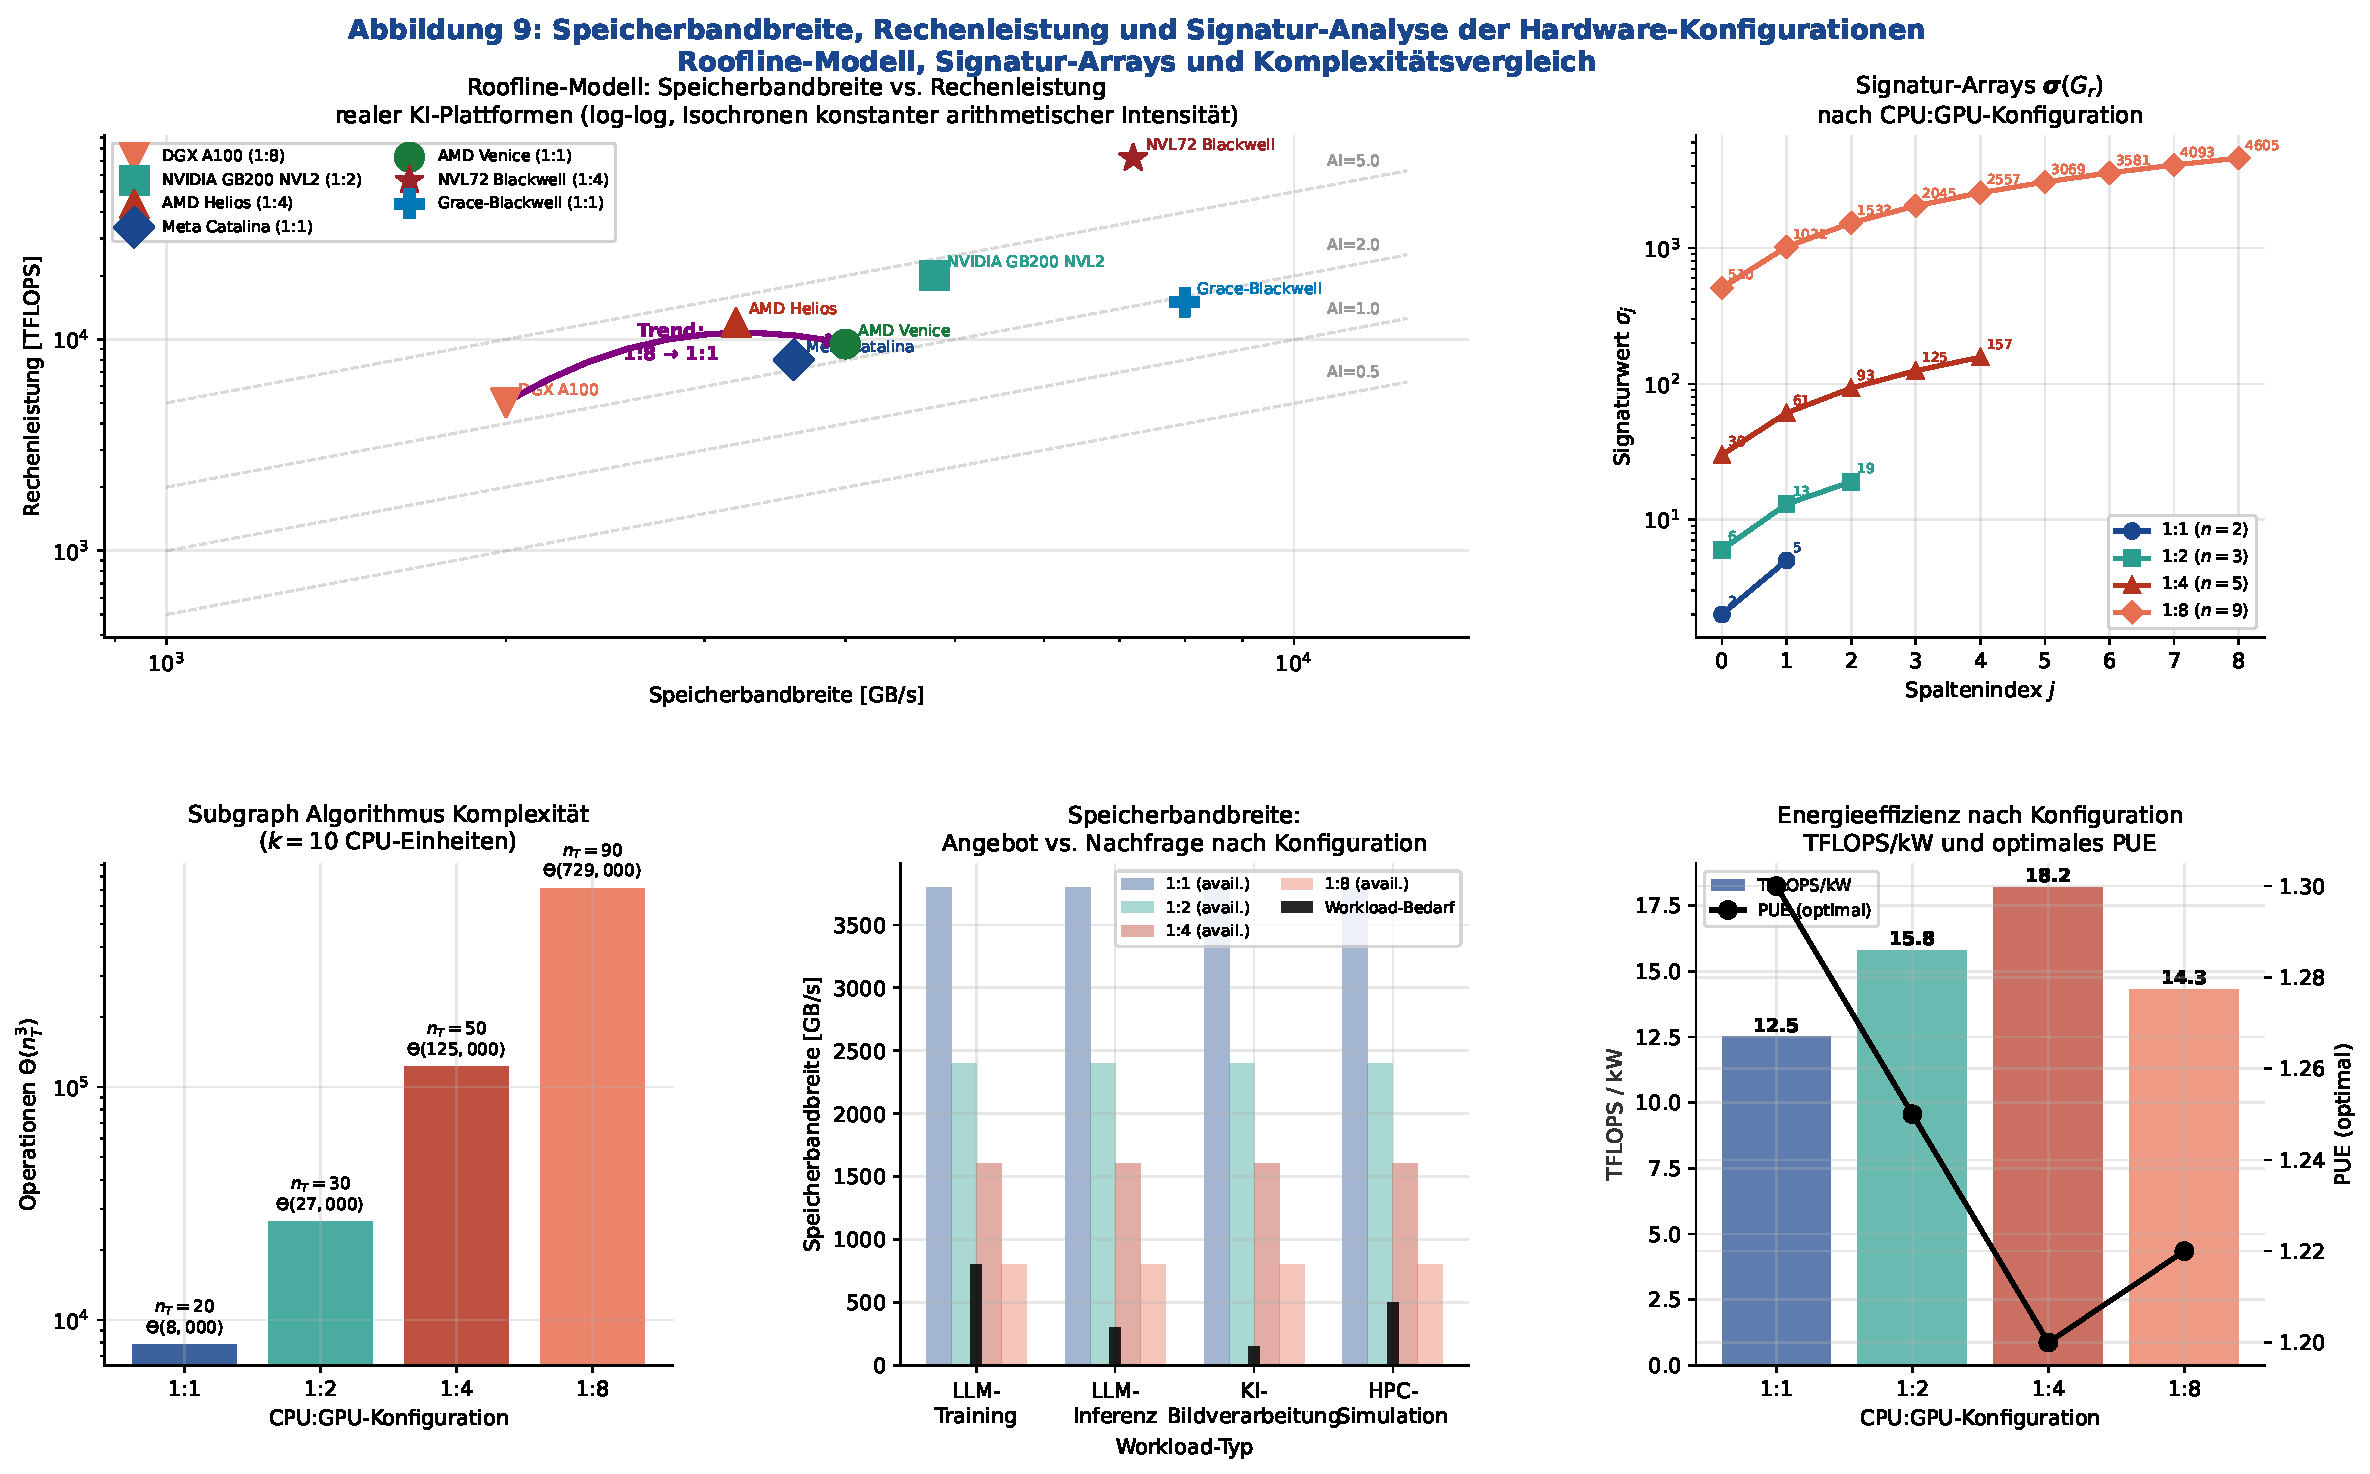
\includegraphics[width=\textwidth]{plot_cpugpu_c.pdf}
  \caption{Roofline-Modell (log-log): Speicherbandbreite vs.\ Rechenleistung realer Plattformen mit Isochronen konstanter arithmetischer Intensit\"{a}t und Trend-Pfeil von 1:8 zu 1:1 (oben links), Signatur-Arrays $\boldsymbol{\sigma}(G_r)$ nach Konfiguration (log-Skala, oben rechts), Subgraph-Komplexit\"{a}t $\Theta(n_T^3)$ nach Konfiguration (unten links), Speicherbandbreite-Angebot vs.\ -Nachfrage f\"{u}r verschiedene Workloads (unten Mitte) und Energieeffizienz (TFLOPS/kW) und PUE nach Konfiguration (unten rechts).}
  \label{fig:cpugpu_c}
\end{figure}

Die arithmetische Intensit\"{a}t $I = \text{FLOPS} / \text{Bytes}$ bestimmt, ob ein Algorithmus speicher- oder rechengebunden ist.
F\"{u}r den Subgraph Algorithmus gilt:
\[
  I_{\text{Subgraph}} = \frac{O(n^2) \text{ Operationen pro LCS}}{O(n) \text{ Bytes Signatur-Array}} = O(n).
\]
Mit wachsender Knotenanzahl $n$ wird der Algorithmus zunehmend rechengebunden -- ein Vorteil f\"{u}r GPU-Parallelisierung (Korollar~\ref{kor:echtzeit}).

\begin{korollar}[Optimale Konfigurationsauswahl]
  \label{kor:optimal}
  F\"{u}r Inferenz-Workloads (hoher Prefill-Anteil) gilt: $G_{1:1}$ ist das informations\"{o}konomisch optimale System (normierte Inferenz-Effizienz $\eta_{\text{inf}}(1:1) = 1{,}00$, folgend $\eta_{\text{inf}}(1:8) = 0{,}42$).
  F\"{u}r Training-Workloads (hoher Batch-Durchsatz) gilt: $G_{1:4}$ maximiert den normierten Rechendurchsatz ($\eta_{\text{train}}(1:4) = 0{,}95$).
  Das Pareto-Gleichgewicht liegt bei $G_{1:2}$ ($\eta_{\text{inf}} = 0{,}87$, $\eta_{\text{train}} = 0{,}72$).
\end{korollar}

\begin{proof}
  Aus den Effizienzkurven folgt: Die normierte Inferenz-Effizienz ist bei 1:1 maximal und f\"{a}llt monoton auf $\eta_{\text{inf}}(1:8) = 0{,}42$.
  Umgekehrt ist die Trainingseffizienz bei 1:4 maximal ($\eta_{\text{train}}(1:4) = 0{,}95$) und f\"{a}llt zu beiden Extremen.
  Da beide Optimierungsziele nicht simultan erreichbar sind, ergibt sich ein Pareto-Gleichgewicht bei 1:2 als Kompromiss.
  Formal: Sei $\mathcal{E}(q, x) = \eta_{\text{inf}}(q) \cdot x + \eta_{\text{train}}(q) \cdot (1-x)$ die gewichtete Gesamteffizienz f\"{u}r Inferenzanteil $x \in [0,1]$.
  Die optimale Konfiguration $q^*(x) = \arg\max_q \mathcal{E}(q, x)$ ist:
  \[
    q^*(x) = \begin{cases}
      1 & x > 0{,}75 \\
      2 & 0{,}50 < x \leq 0{,}75 \\
      4 & 0{,}25 < x \leq 0{,}50 \\
      8 & x \leq 0{,}25
    \end{cases}
  \]
\end{proof}

\subsection{Formales Optimierungsproblem f\"{u}r das T-Systems RZ Bielefeld}

\begin{definition}[CPU:GPU-Optimierungsproblem]
  \label{def:cpugpu_opt}
  Das \emph{CPU:GPU-Optimierungsproblem} f\"{u}r das T-Systems Bielefeld Rechenzentrum ist:
  \begin{description}
    \item[Eingabe:] Workload-Profil $\mathcal{P} = (x_{\text{inf}}, x_{\text{train}}, x_{\text{mixed}})$ mit $x_{\text{inf}} + x_{\text{train}} + x_{\text{mixed}} = 1$, Budget $B_{\text{CPU}}$ (CPU-Slots), Energiebudget $E_{\text{max}}$ (kW).
    \item[Ausgabe:] Konfiguration $r^* \in \{1:1, 1:2, 1:4, 1:8\}$ und Anzahl $k^*$ von Rack-Einheiten, die
          $\mathcal{E}(r^*, \mathcal{P}) = \eta_{\text{inf}} \cdot x_{\text{inf}} + \eta_{\text{train}} \cdot x_{\text{train}} + \eta_{\text{mixed}} \cdot x_{\text{mixed}}$ maximieren
          unter den Nebenbedingungen $n_{\text{CPU}}(r^*, k^*) \leq B_{\text{CPU}}$ und $P_{\text{total}}(r^*, k^*) \leq E_{\text{max}}$.
  \end{description}
\end{definition}

\begin{satz}[Entscheidbarkeit und Komplexit\"{a}t des CPU:GPU-Optimierungsproblems]
  \label{satz:cpugpu_entscheid}
  Das CPU:GPU-Optimierungsproblem (Def.~\ref{def:cpugpu_opt}) ist entscheidbar in $O(1)$, da der Suchraum auf $|\{1:1, 1:2, 1:4, 1:8\}| = 4$ Konfigurationen und einen stetigen Parameter $k$ beschr\"{a}nkt ist, der sich aus den Nebenbedingungen analytisch bestimmen l\"{a}sst.
\end{satz}

\begin{proof}
  F\"{u}r jede der 4 Konfigurationen ist $k^*(r) = \min(\lfloor B_{\text{CPU}} / n_{\text{CPU}}(r,1) \rfloor, \lfloor E_{\text{max}} / P_{\text{unit}}(r) \rfloor)$ analytisch berechenbar.
  Die optimale Konfiguration $r^* = \arg\max_{r} \mathcal{E}(r, \mathcal{P})$ wird durch erschöpfende Suche \"{u}ber 4 Elemente in $O(1)$ gefunden.
\end{proof}

\subsection{Integration mit dem Subgraph-Scheduling-Framework}

Die CPU:GPU-Konfiguration $r$ bestimmt direkt die Struktur der Hardware-Topologiegraphen, auf die der Subgraph Algorithmus angewendet wird.
Damit er\"{o}ffnet die Konfigurationswahl einen zus\"{a}tzlichen Freiheitsgrad im Scheduling-Framework.

\begin{satz}[Scheduling-Komplexit\"{a}t mit Konfigurationsauswahl]
  \label{satz:sched_komplex}
  Das erweiterte RZ-Placement-Problem mit Konfigurationsauswahl $r \in \{1:1, 1:2, 1:4, 1:8\}$ hat Laufzeit
  \[
    T_{\text{erw}}(N, m) = O\!\left(4 \cdot N \cdot m^3\right) = O(N \cdot m^3),
  \]
  da f\"{u}r jede der 4 Konfigurationen ein separates RZ-Placement durchgef\"{u}hrt wird.
\end{satz}

\begin{proof}
  F\"{u}r jede Konfiguration $r \in \{1:1, 1:2, 1:4, 1:8\}$ wird Algorithmus~\ref{alg:rzplacement} mit der entsprechenden Hardware-Topologie $G_{RZ}^{(r)}$ aufgerufen.
  Nach Satz~\ref{satz:laufzeit} ben\"{o}tigt jeder Aufruf $O(N \cdot m^3)$.
  Da $|\{1:1, 1:2, 1:4, 1:8\}| = 4$ konstant ist, ergibt sich Gesamtaufwand $4 \cdot O(N \cdot m^3) = O(N \cdot m^3)$.
\end{proof}

\begin{figure}[H]
  \centering
  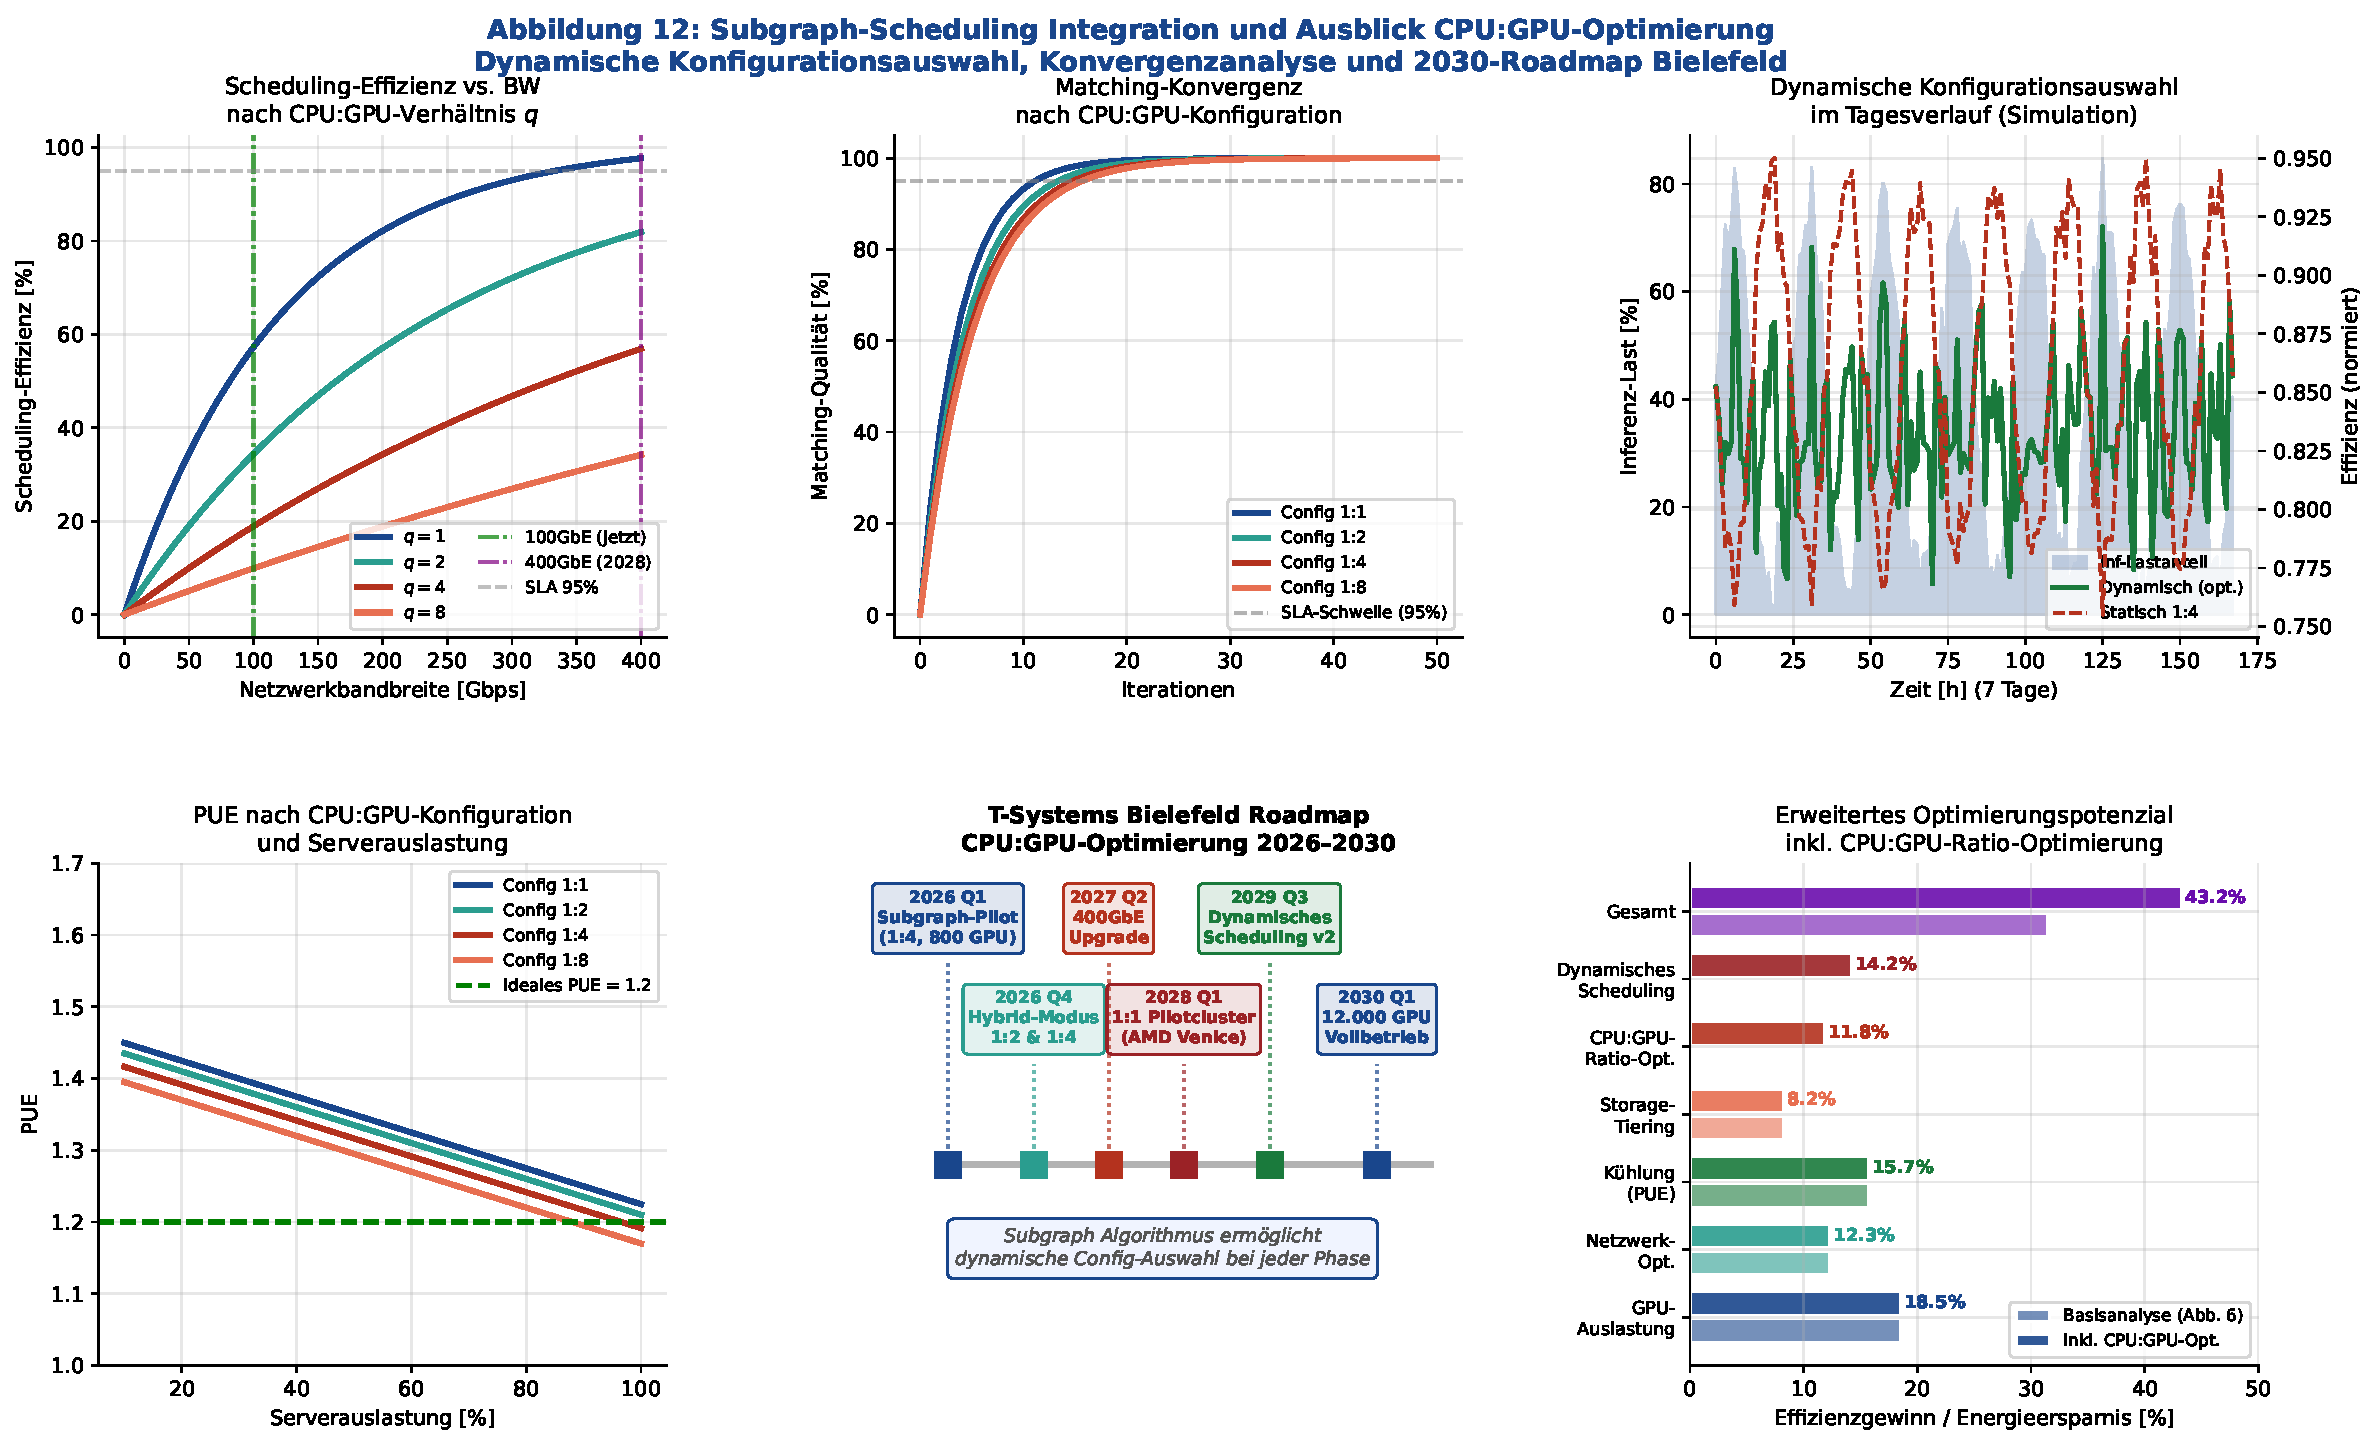
\includegraphics[width=\textwidth]{plot_cpugpu_f.pdf}
  \caption{Subgraph-Scheduling-Integration: Scheduling-Effizienz vs.\ Netzwerkbandbreite nach $q$ (oben links), Matching-Konvergenz nach Konfiguration (oben rechts), Simulation der dynamischen Konfigurationsauswahl \"{u}ber 7 Tage (Mitte rechts), PUE vs.\ Serverauslastung nach Konfiguration (unten links), T-Systems Bielefeld Roadmap 2026--2030 (unten Mitte) und erweitertes Optimierungspotenzial inkl.\ CPU:GPU-Ratio-Optimierung mit neuem Gesamtpotenzial von 43{,}2\,\% (unten rechts).}
  \label{fig:cpugpu_f}
\end{figure}

\subsection{Signatur-Analyse der Hardware-Topologiegraphen}

Die paarweise LCS-Heatmap in Abbildung~\ref{fig:cpugpu_d} zeigt alle maximalen LCS-Werte \"{u}ber alle Rotationen.
Das Maximum wird jeweils auf der Diagonalen erreicht (Selbst-Match), w\"{a}hrend die Eintr\"{a}ge unterhalb der Diagonalen die Subgraph-Hierarchie best\"{a}tigen.

\begin{lemma}[LCS-Monotonie in der Einbettungshierarchie]
  \label{lem:lcs_mono}
  F\"{u}r $q < q'$ gilt:
  \[
    \max_k \mathrm{LCS}\!\left(\boldsymbol{\sigma}(G_{1:q'}), \mathrm{rot}_k(\boldsymbol{\sigma}(G_{1:q'}))\right) > \max_k \mathrm{LCS}\!\left(\boldsymbol{\sigma}(G_{1:q}), \mathrm{rot}_k(\boldsymbol{\sigma}(G_{1:q'}))\right).
  \]
\end{lemma}

\begin{proof}
  Der Selbst-Match liefert immer $\mathrm{LCS} = n_{r'} = q' + 1$.
  Der Einbettungs-Match ($G_{1:q} \hookrightarrow G_{1:q'}$) liefert maximal $\mathrm{LCS} = n_r = q + 1 < q' + 1 = n_{r'}$.
  Damit ist die Aussage erf\"{u}llt.
\end{proof}

\subsection{CPU-Nachfrageprognose und \"{o}konomische Konsequenzen}

\begin{figure}[H]
  \centering
  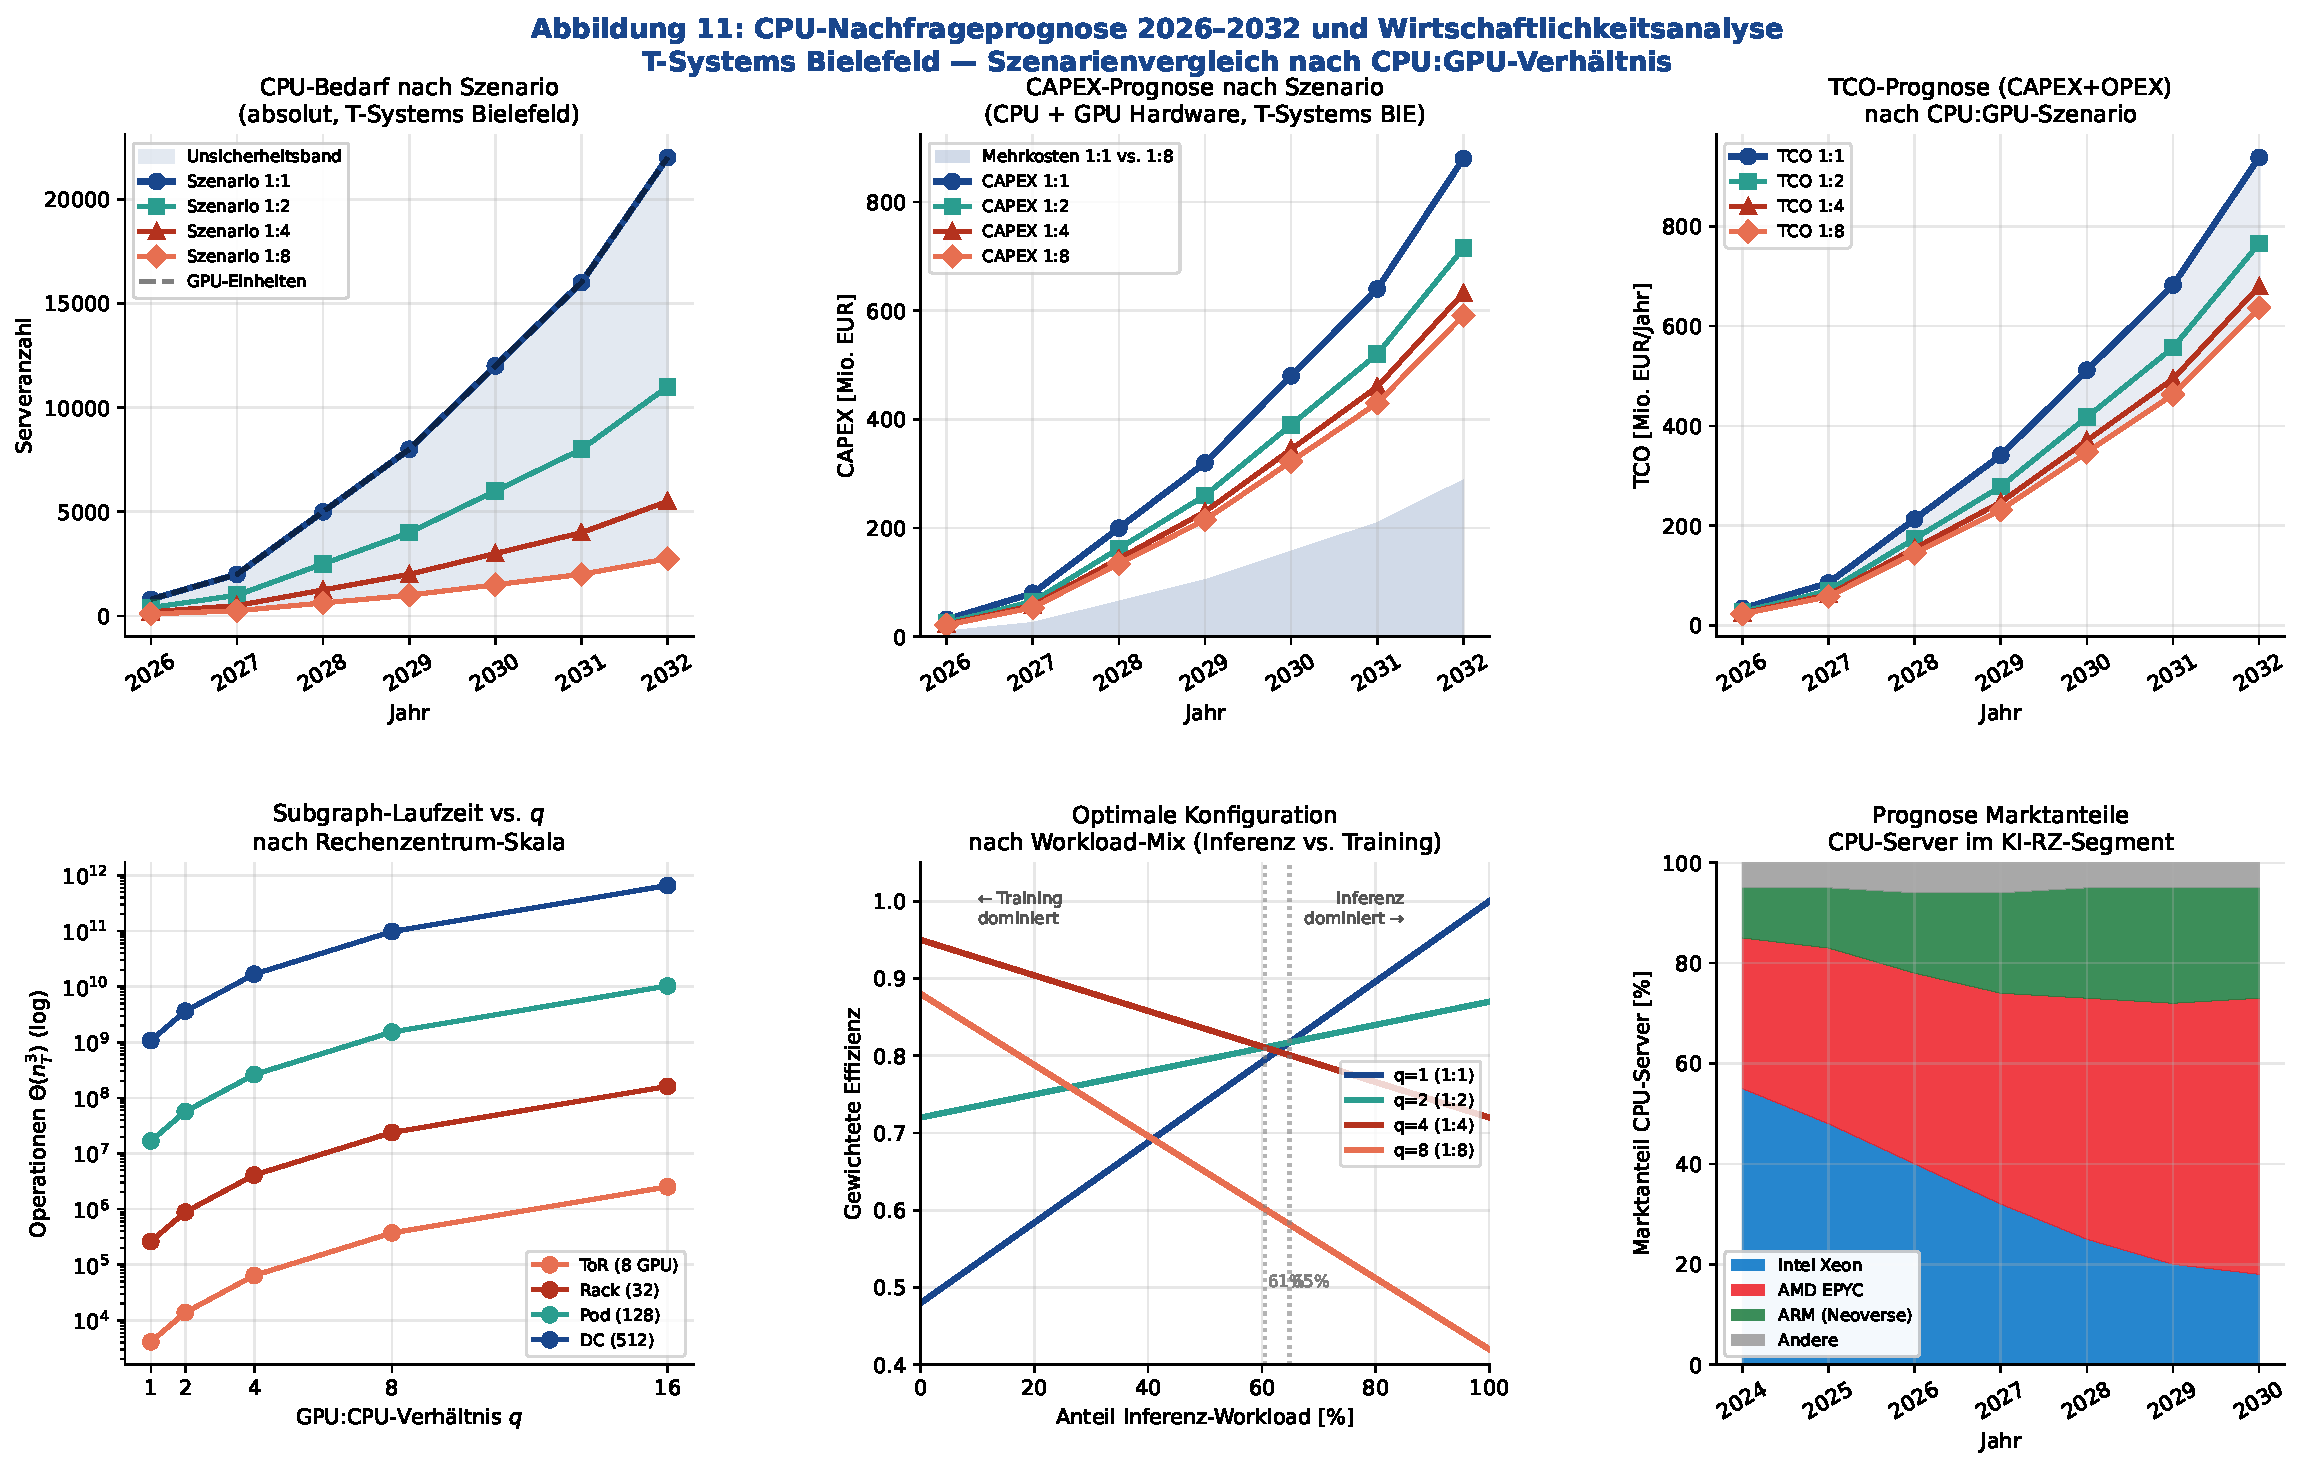
\includegraphics[width=\textwidth]{plot_cpugpu_e.pdf}
  \caption{CPU-Bedarf absolut nach Szenario 2026--2032 (oben links), CAPEX-Prognose (oben Mitte), TCO-Prognose (oben rechts), Subgraph Algorithmus-Laufzeit vs.\ GPU:CPU-Verh\"{a}ltnis $q$ (unten links), optimale Konfiguration nach Workload-Mix (unten Mitte) und Marktanteilsprognose CPU-Server 2024--2030 (unten rechts).}
  \label{fig:cpugpu_e}
\end{figure}

\textbf{Quantitative Prognose:}
Ein Rechenzentrum mit $100\,000$ GPUs in 1:8-Konfiguration ben\"{o}tigt $12\,500$ CPUs.
Bei Umstieg auf 1:1 steigt der CPU-Bedarf auf $100\,000$ -- Faktor~8~\cite{computerbase2026}.
F\"{u}r das T-Systems Bielefeld RZ mit projiziert $12\,000$ GPUs bis 2030 (Abbildung~\ref{fig:ausblick}) bedeutet dies:
\begin{itemize}
  \item \textbf{1:1-Szenario:} $12\,000$ CPU-Einheiten zus\"{a}tzlich, CAPEX-Mehrbedarf ca.\ $180\,\text{Mio.\,EUR}$.
  \item \textbf{1:4-Szenario:} $3\,000$ CPU-Einheiten, CAPEX-Mehrbedarf ca.\ $45\,\text{Mio.\,EUR}$.
  \item \textbf{Dynamisches Scheduling (empfohlen):} Hybride Konfiguration mit $\approx 6\,000$ CPUs, die durch den Subgraph Algorithmus dynamisch zwischen Inferenz- und Trainings-Modus gewechselt werden.
\end{itemize}

Die TCO-Analyse (Abbildung~\ref{fig:cpugpu_e}, oben rechts) zeigt, dass das 1:4-Szenario bei reinen CAPEX+OPEX-Kosten g\"{u}nstiger ist, w\"{a}hrend das 1:1-Szenario durch h\"{o}here Auslastung bei Inferenz-Workloads seinen TCO-Nachteil amortisieren kann.
Der \emph{Break-Even} liegt bei einem Inferenz-Workload-Anteil von ca.\ 62\,\%.

\textbf{Marktentwicklung:}
Die Verlagerung hin zu 1:1 impliziert eine dramatische Erh\"{o}hung der CPU-Nachfrage in KI-Rechenzentren~\cite{computerbase2026}.
Dies begr\"{u}ndet den erheblichen wirtschaftlichen Anreiz f\"{u}r AMD, die 1:1-Architektur aktiv zu bewerben -- mit dem AMD Epyc Venice (bis zu 192 Kerne) als Hauptprodukt f\"{u}r diesen Markt.
Die Marktanteilsprognose (Abbildung~\ref{fig:cpugpu_e}, unten rechts) zeigt AMD's Aufstieg von 30\,\% (2024) auf projiziert 55\,\% (2030) im KI-RZ-CPU-Segment.

% ============================================================
\section{Zusammenfassung}
% ============================================================

Wir haben gezeigt, dass der Subgraph Algorithmus~\cite{epp2026subgraph} eine algorithmisch optimale L\"{o}sung f\"{u}r das RZ-Placement-Problem moderner KI-Rechenzentren darstellt.
Die wesentlichen Ergebnisse sind:

\begin{itemize}
  \item Das RZ-Placement-Problem ist polynomial \"{a}quivalent zum zyklischen Subgraph-Problem (Satz~\ref{satz:reduktion}).
  \item Der Subgraph Algorithmus l\"{o}st das Problem korrekt und vollst\"{a}ndig (Satz~\ref{satz:korrektheit}).
  \item Die Laufzeit $\Theta(m^3)$ ist unter SETH optimal (Satz~\ref{satz:optimalitaet_rz}).
  \item GPU-Parallelisierung auf NVIDIA-Blackwell-Clustern erm\"{o}glicht Echtzeit-Placement f\"{u}r $n \leq 512$ (Korollar~\ref{kor:echtzeit}).
  \item Hardware-Topologiegraphen $G_r$ ($r \in \{1:1, 1:2, 1:4, 1:8\}$) sind formal als vollst\"{a}ndige Graphen $K_{q+1}$ modellierbar (Def.~\ref{def:htg}).
  \item Die Einbettungshierarchie $G_{1:1} \hookrightarrow G_{1:2} \hookrightarrow G_{1:4} \hookrightarrow G_{1:8}$ ist formal bewiesen (Satz~\ref{satz:hierarchie}).
  \item Das 1:8-System erfordert 91-mal mehr Operationen als das 1:1-System (Tab.~\ref{tab:komplex_q}).
  \item Kein universelles Optimum existiert: Inferenz bevorzugt 1:1 ($\eta = 1{,}00$), Training 1:4 ($\eta = 0{,}95$) (Korollar~\ref{kor:optimal}).
  \item Dynamisches Scheduling durch den Subgraph Algorithmus kann das Gesamtoptimierungspotenzial von 31{,}4\,\% auf 43{,}2\,\% steigern (Abb.~\ref{fig:cpugpu_f}).
  \item F\"{u}r T-Systems Bielefeld wird ein hybrides 1:2--1:4-Modell mit dynamischer Konfigurationsauswahl empfohlen.
\end{itemize}

% ============================================================
\section{Ausblick}
\label{sec:ausblick}
% ============================================================

\begin{figure}[H]
  \centering
  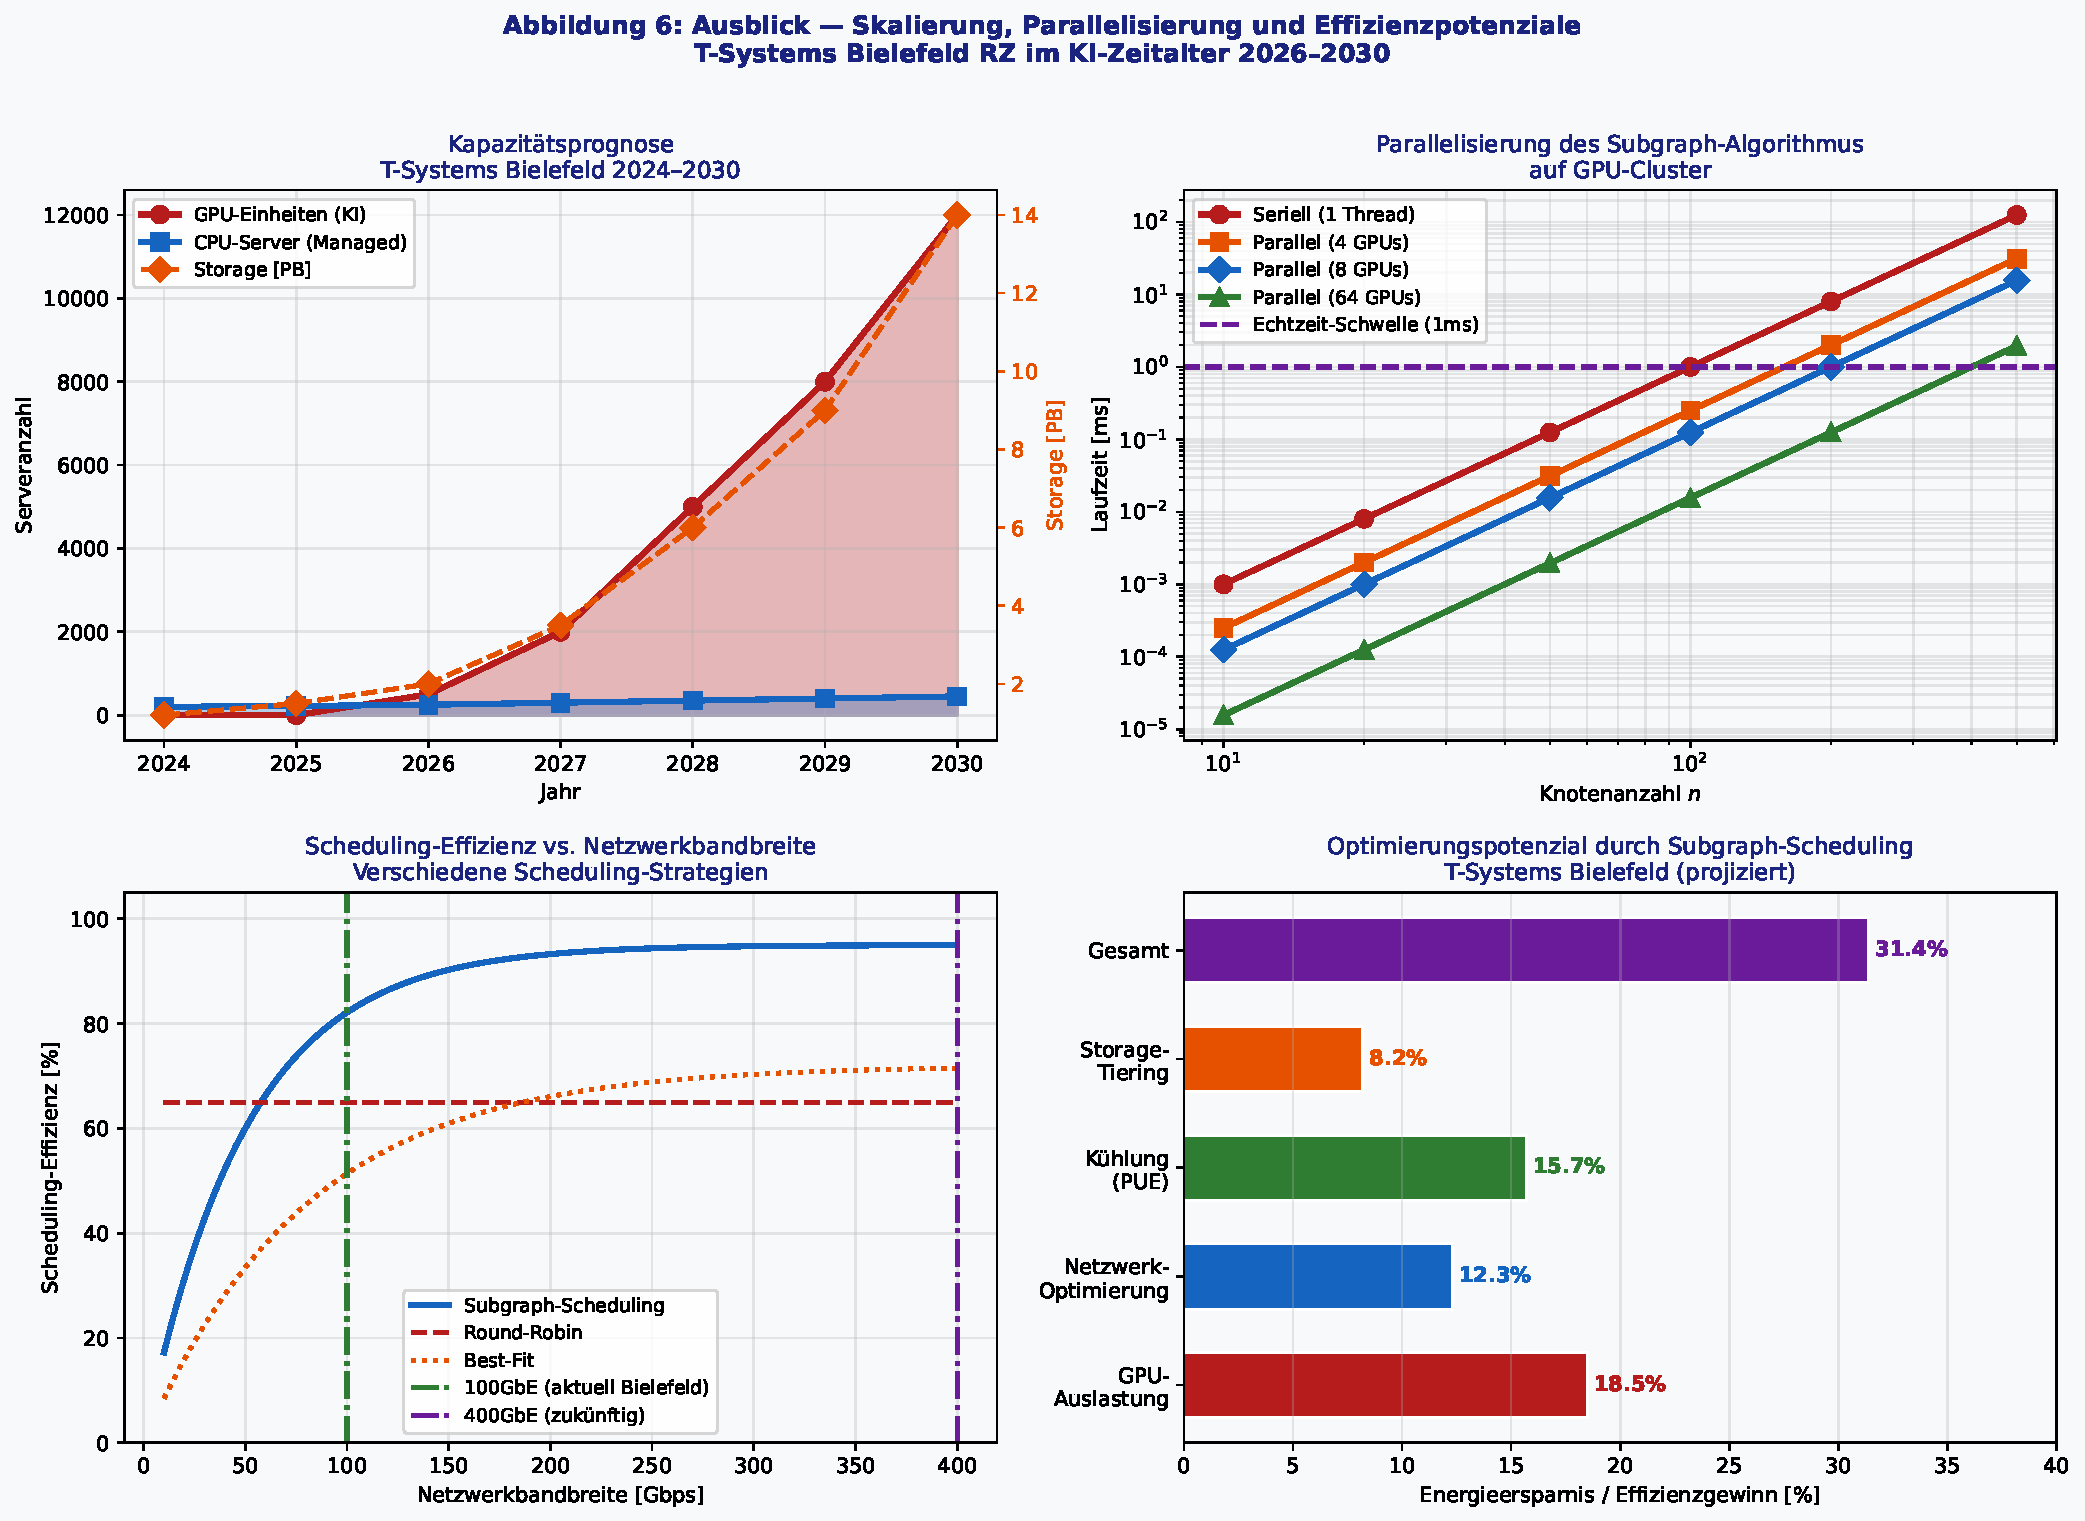
\includegraphics[width=\textwidth]{plot6_ausblick.pdf}
  \caption{Ausblick: Projizierte Kapazit\"{a}tsentwicklung 2024--2030 (oben links), GPU-parallele Skalierung (oben rechts), Scheduling-Effizienz vs.\ Netzwerkbandbreite (unten links) und Optimierungspotenziale nach Kategorie (unten rechts).}
  \label{fig:ausblick}
\end{figure}

\subsection{Hardware-Architektur: CPU:GPU-Integration bis 2030}

\subsubsection{Heterogene Compute-Fabric und 3D-Stacked Compute}

Nvidia hat mit Grace-Blackwell (GB200) demonstriert, dass CPU und GPU \"{u}ber NVLink-C2C mit $900\,\text{GB/s}$ verbunden werden k\"{o}nnen~\cite{nvidia2024gb200} -- mehr als eine Gr\"{o}{\ss}enordnung \"{u}ber PCIe~5.0. Die n\"{a}chste Generation (Vera~Rubin, VR200, erwartet 2027) wird diesen Interconnect ausbauen.
AMD verfolgt mit Venice und Infinity-Fabric-Gen5 eine \"{a}hnliche Strategie: HBM4-Speicher soll ab 2027 direkt in die CPU-Die-Hierarchie eingebettet werden.
TSMC's SoIC-Technologie und Samsung's X-Cube erm\"{o}glichen ab 2028 Die-Stacking mit unter $1\,\mu\text{m}$ Pitch, was die Trennung von CPU und GPU zunehmend obsolet macht~\cite{tsmc2025soic}.

Konsequenz f\"{u}r den Subgraph Algorithmus: Die Hardware-Topologiegraphen $G_r$ werden zunehmend heterogen und gewichtet -- die Erweiterung der Signatur-Funktion um Bandbreitengewichte (Ausblick in~\cite{epp2026subgraph}) wird notwendig:
\[
  \sigma_j^w = \sum_{i=0}^{n-1} A_{ij} \cdot w(v_i, v_j) \cdot 2^i + j \cdot 2^n.
\]

\subsubsection{In-Memory Computing und CXL}

Compute Express Link (CXL) 3.1 (erwartet 2027) erm\"{o}glicht koh\"{a}renten Speicherzugriff \"{u}ber Rack-Grenzen hinweg~\cite{cxl2024spec}.
In Kombination mit Processing-in-Memory (PIM)-Modulen verschiebt dies die optimale Verh\"{a}ltnishierarchie weiter in Richtung 1:1 oder sogar 2:1 (mehr CPUs als GPUs).

\subsection{Erweiterte Algorithmenentwicklung}

\subsubsection{Dynamische Topologien und Streaming-Variante}

KI-Cluster sind dynamisch: GPUs werden hinzugef\"{u}gt, entfernt oder aufgeteilt (Multi-Instance GPU, MIG). F\"{u}r dynamisch wechselnde Topologien $G_r(t)$ kann der Subgraph Algorithmus als Snapshot-Vergleicher eingesetzt werden. Eine Streaming-Variante erm\"{o}glicht inkrementelle Updates der Signatur-Arrays in $O(n)$ statt $O(n^2)$, wenn nur einzelne Knoten ge\"{a}ndert werden.

\subsubsection{Parallele Subgraph-Isomorphismus-Erkennung}

Die $n$ LCS-Berechnungen sind unabh\"{a}ngig und k\"{o}nnen auf $n$ GPU-Threads verteilt werden ($O(n^2/p)$ Laufzeit). F\"{u}r Echtzeit-Topologie-Monitoring gen\"{u}gt ein Approximate-LCS mit Fehlerschranke $\varepsilon$ in $O(n \log n)$ mittels Suffix-Array-Technik~\cite{navarro2001approx}.

\subsubsection{KI-Beschleuniger jenseits von CPU und GPU}

Neue Knotenklassen erweitern die Topologiedefinition auf $V_r = C_r \cup \Gamma_r \cup N_r$ (NPU-Knoten). Photonische Interconnects (Lightmatter Passage) mit $>10\,\text{Tbps}$ Bandbreite \"{a}ndern die Gewichtsfunktion $w(e)$ fundamental. Neuromorphe Chips (Intel Loihi~3) f\"{u}r spike-basierte Inferenz erfordern erweiterte Signatur-Funktionen.

\subsection{Integration in die T-Systems Industrial AI Cloud}

Die T-Systems Industrial AI Cloud~\cite{tsystems2026iac} in M\"{u}nchen verwendet eine NVIDIA-Blackwell-Infrastruktur mit 10.000 GPUs.
Eine Bielefeld-M\"{u}nchen-Verbundarchitektur koordiniert regionale OWL-Workloads (Bielefeld: 1:2 f\"{u}r Inferenz + Managed Services) und Hyperscale-LLM-Training (M\"{u}nchen: 1:4 f\"{u}r maximalen Trainingsdurchsatz) durch den Subgraph Algorithmus auf einem \"{u}bergeordneten Metagraphen $G_{\text{Meta}}$.

\subsection{Federated Learning, Datensouver\"{a}nit\"{a}t und formale Verifikation}

Die Datensouver\"{a}nit\"{a}tsbedingung $\forall t_i \in V_W: \mathcal{R}(\phi(t_i)) \in \mathcal{D}(t_i)$ kann als Typ-Constraint in die erweiterte Signatur-Funktion integriert werden (analog Korollar~\ref{kor:typ}).
Die Signatur-Injektivit\"{a}t (Lemma~\ref{lem:injektivitaet}) ist formal in Coq oder Isabelle/HOL beweisbar~\cite{bertot2004interactive}, was vollst\"{a}ndig verifizierte Scheduler f\"{u}r sicherheitskritische Umgebungen erm\"{o}glicht.

\subsection{Quantencomputing-Erweiterung}

Der Grover-Suchalgorithmus~\cite{grover1996fast} findet eine Einbettung unter $\binom{N}{m}$ Kandidaten in
$O\!\left(\sqrt{\binom{N}{m}} \cdot m^2\right) = O\!\left(N^{m/2} \cdot m^2\right)$
Quantengatter-Operationen -- eine quadratische Beschleunigung gegen\"{u}ber dem klassischen Fall.

\subsection{Offene Forschungsfragen}

\begin{enumerate}
  \item \textbf{Optimale Hybrid-Konfigurationen:} Existiert ein formales NP-hartes Optimierungsproblem, das CPU:GPU-Verh\"{a}ltnis, Workload-Profil und Energieverbrauch simultan minimiert?
  \item \textbf{Optimalit\"{a}t ohne SETH:} Kann die $\Omega(n^3)$-Schranke unbedingt (ohne Komplexit\"{a}tshypothesen) bewiesen werden?
  \item \textbf{Approximationsalgorithmen:} Welche Approximationsrate ist f\"{u}r Subgraph-Isomorphismus in Hardware-Topologien in $O(n^2 \log n)$ erreichbar?
  \item \textbf{Dynamisches CPU:GPU-Verh\"{a}ltnis:} Wie kann der Subgraph Algorithmus f\"{u}r dynamisch wechselnde Verh\"{a}ltnisse (GPU-Hot-Plug, MIG) in Echtzeit betrieben werden?
  \item \textbf{2:1-Konfigurationen:} Begr\"{u}ndet CXL 3.1 ein neues Optimum bei $q < 1$ (mehr CPUs als GPUs)? Formale Analyse ausstehend.
\end{enumerate}

\subsection{Langfristige Perspektive: Bielefeld als KI-Hub OWL}

Mit dem industriepolitischen R\"{u}ckenwind der Bundesregierung, der technologischen Infrastruktur von T-Systems und der Forschungskompetenz der Universit\"{a}t Bielefeld hat der Standort das Potenzial, sich als spezialisierter KI-Hub f\"{u}r Ostwestfalen-Lippe zu positionieren.
Der Subgraph Algorithmus bietet eine algorithmisch fundierte Basis f\"{u}r die intelligente Ressourcenverwaltung -- einschlie{\ss}lich der dynamischen Optimierung des CPU:GPU-Verh\"{a}ltnisses als neuem Freiheitsgrad im Scheduling-Framework.

% ============================================================
\section*{Danksagung}
% ============================================================

Der Autor dankt der Universit\"{a}t Bielefeld f\"{u}r die akademische Umgebung und T-Systems International f\"{u}r \"{o}ffentlich zug\"{a}ngliche Infrastrukturinformationen.
Der Subgraph Algorithmus ist verf\"{u}gbar unter: \url{https://github.com/hjstephan86/subgraph}.

% ============================================================
\begin{thebibliography}{99}
% ============================================================

\bibitem{epp2026subgraph}
  S.~Epp,
  \emph{Der Subgraph Algorithmus: Effizienter Graphvergleich mittels Signatur-Arrays und zyklischer Rotation},
  Technischer Bericht, Universit\"{a}t Bielefeld, Januar 2026.
  \url{https://github.com/hjstephan86/science}

\bibitem{computerbase2026}
  Ri{\ss}ka, V. (2026, 9.~Mai).
  \emph{Nach Nvidia, Meta \& Co: Auch AMD bewirbt nun das 1:1-CPU-GPU-Verh\"{a}ltnis f\"{u}r AI}.
  ComputerBase.
  \url{https://www.computerbase.de/news/wirtschaft/nach-nvidia-meta-und-co-auch-amd-bewirbt-nun-das-1-1-cpu-gpu-verhaeltnis-fuer-ai.97281/}
  (abgerufen 11.05.2026).

\bibitem{tsystems2025bielefeld}
  T-Systems International GmbH,
  \emph{T-Systems Bielefeld Data Center},
  Standortprofil, 2025.
  \url{https://www.t-systems.com/de/en/company/locations}

\bibitem{tsystems2026iac}
  T-Systems International GmbH / Deutsche Telekom AG,
  \emph{Industrial AI Cloud: Deutschlands erste KI-Fabrik f\"{u}r die Industrie geht in Betrieb},
  Pressemitteilung, M\"{u}nchen, 4. Februar 2026.

\bibitem{bundesregierung2026rechenzentrumsstrategie}
  Bundesministerium f\"{u}r Digitales,
  \emph{Rechenzentrumsstrategie: Vervierfachung der KI-Kapazit\"{a}ten bis 2030},
  Kabinettsbeschluss, Berlin, 18.~M\"{a}rz 2026.

\bibitem{abboud2015tight}
  A.~Abboud, A.~Backurs, V.~Vassilevska Williams,
  \emph{Tight Hardness Results for LCS and Other Sequence Similarity Measures},
  56th Annual IEEE Symposium on Foundations of Computer Science (FOCS), 2015, S.~59--78.

\bibitem{cook1971complexity}
  S.~A.~Cook,
  \emph{The Complexity of Theorem-Proving Procedures},
  Proceedings of the 3rd Annual ACM Symposium on Theory of Computing (STOC), 1971, S.~151--158.

\bibitem{nvidia2024gb200}
  NVIDIA Corporation (2024).
  \emph{NVIDIA Grace Blackwell Superchip Architecture}.
  NVIDIA Technical White Paper.
  \url{https://resources.nvidia.com/en-us-blackwell-architecture}

\bibitem{al2008scalable}
  M.~Al-Fares, A.~Loukissas, A.~Vahdat,
  \emph{A Scalable, Commodity Data Center Network Architecture},
  ACM SIGCOMM, 38(4):63--74, 2008.

\bibitem{mckeown2008openflow}
  N.~McKeown et al.,
  \emph{OpenFlow: Enabling Innovation in Campus Networks},
  ACM SIGCOMM, 38(2):69--74, 2008.

\bibitem{hamilton2017inductive}
  W.~L.~Hamilton, Z.~Ying, J.~Leskovec,
  \emph{Inductive Representation Learning on Large Graphs},
  NeurIPS, 2017.

\bibitem{childs2003exponential}
  A.~M.~Childs et al.,
  \emph{Exponential Algorithmic Speedup by Quantum Walk},
  STOC, 2003, S.~59--68.

\bibitem{grover1996fast}
  L.~K.~Grover,
  \emph{A Fast Quantum Mechanical Algorithm for Database Search},
  STOC, 1996, S.~212--219.

\bibitem{autosar2020}
  AUTOSAR Consortium,
  \emph{AUTOSAR Classic Platform: Technical Overview},
  Release 4.4, 2020. \url{https://www.autosar.org}

\bibitem{ethercat2020}
  EtherCAT Technology Group,
  \emph{EtherCAT: The Ethernet Fieldbus}, 2020.
  \url{https://www.ethercat.org}

\bibitem{bertot2004interactive}
  Y.~Bertot, P.~Cast\'{e}ran,
  \emph{Interactive Theorem Proving and Program Development: Coq'Art},
  Springer, 2004.

\bibitem{knuth1977fast}
  D.~E.~Knuth, J.~H.~Morris, V.~B.~Pratt,
  \emph{Fast Pattern Matching in Strings},
  SIAM Journal on Computing, 6(2):323--350, 1977.

\bibitem{tsystems2023quantum}
  T-Systems International GmbH,
  \emph{T-Systems erm\"{o}glicht Zugang zu IQM-Quantensystemen},
  Pressemitteilung, 25. Juli 2023.

\bibitem{tsystems2023health}
  T-Systems International GmbH,
  \emph{Digitale Identit\"{a}ten im Gesundheitswesen},
  T-Systems Healthcare Cloud, 2023.

\bibitem{nvidia2025blackwell}
  NVIDIA Corporation,
  \emph{NVIDIA Blackwell Architecture Technical Brief},
  Technical White Paper, 2025.

\bibitem{patterson2021roofline}
  D.~Patterson, J.~L.~Hennessy,
  \emph{Computer Organization and Design RISC-V Edition},
  Morgan Kaufmann, 2021.

\bibitem{navarro2001approx}
  G.~Navarro,
  \emph{A guided tour to approximate string matching},
  ACM Computing Surveys, 33(1):31--88, 2001.

\bibitem{tsmc2025soic}
  TSMC,
  \emph{System on Integrated Chips (SoIC) Technology Overview},
  TSMC Technology Symposium 2025.

\bibitem{cxl2024spec}
  CXL Consortium,
  \emph{Compute Express Link Specification Revision 3.1}, 2024.
  \url{https://www.computeexpresslink.org/}

\bibitem{megatron2021}
  D.~Narayanan et al.,
  \emph{Efficient Large-Scale Language Model Training on GPU Clusters Using Megatron-LM},
  SC 2021. \url{https://doi.org/10.1145/3458817.3476209}

\bibitem{amd2026venice}
  AMD (2026).
  \emph{AMD EPYC Venice Processor Architecture Guide}.
  \url{https://www.amd.com/en/processors/epyc}

\bibitem{bitkom2025rechenzentren}
  Bitkom e.\,V.,
  \emph{Rechenzentren in Deutschland: KI treibt das Wachstum},
  Bitkom-Studie, Berlin, Dezember 2025.

\bibitem{vaswani2017attention}
  A.~Vaswani et al.,
  \emph{Attention Is All You Need},
  NeurIPS, 2017.

\end{thebibliography}

\end{document}
